\documentclass{scrbook}
\usepackage{graphicx} % Required for inserting images
\usepackage{tabularx} % Required for fixed width tables
\usepackage{scrlayer-scrpage} % Required for the subtitles
\usepackage{url} % Required for the URLs
\usepackage{hyperref} % Required for the URLs
\usepackage{listings} % Required for the code snippets
\usepackage{mathtools} % Required for the system of equations

\usepackage{tikz} % Required for the vector graphics
\usepackage{enumitem} % Required for custom enumerations

\usepackage{inconsolata}
% Put the caption of the snippets at the bottom
\lstset{
    captionpos=b,
    basicstyle=\ttfamily\small,
    columns=fullflexible
}


\title{JavaScript 2}
\subtitle{Ambient intelligence course (A.Y. 2025/2026)\\Topic taught by Prof. Davide Loconte}
\author{Gabriele Colapinto}
\date{\today}

\begin{document}

\maketitle
\thispagestyle{empty}

{\Large\textbf{License}} \\
{Notes from Ambient intelligence (A.Y. 2025/2026) by Gabriele Colapinto. 
Course taught by professors Michele Ruta, Floriano Scioscia, Arnaldo Tomasino, Davide Loconte — 
Licensed under CC BY-NC 4.0.\\
\url{https://creativecommons.org/licenses/by-nc/4.0/}}

\vspace*{\fill}
\rule{\textwidth}{0.2pt}
\small{© 2025 Gabriele Colapinto \\
Released under the \href{https://creativecommons.org/licenses/by-nc/4.0/}{Creative Commons Attribution–NonCommercial 4.0 International License}}

\clearpage

\tableofcontents

\chapter{The Core of JavaScript Objects: Prototypes}

To truly understand inheritance in JavaScript, one must first grasp the concept that lies at its very foundation: the prototype. Unlike classical object-oriented languages that rely on classes, JavaScript is built upon the idea of prototypal inheritance. Every object in JavaScript has a direct link to another object, its prototype, from which it can inherit properties and methods. This simple yet powerful mechanism is the key to understanding how objects relate to and share behavior with one another. \\

A JavaScript prototype is an object from which other objects inherit properties. When you create a function or an object, JavaScript automatically adds a hidden property that points to this prototype object, establishing a link that forms the basis of the inheritance model. Understanding the distinction between the properties used to manage this system—\texttt{prototype} and \texttt{\_\_proto\_\_}—is crucial.

\section{\texttt{prototype} vs. \texttt{\_\_proto\_\_}}

While their names are similar, these two properties serve different functions in the prototypal inheritance system.

\begin{center}
    \begin{tabular}{|p{0.2\linewidth}|p{0.25\linewidth}|p{0.45\linewidth}|}
    \hline    
        Property & Exists On & Purpose \\ \hline
        
        \texttt{\textbf{prototype}} &
        Functions and Classes &
        An object that serves as a \textbf{blueprint} for all instances created from the function or class. Methods and properties added here are shared among all instances. \\ \hline
        
        \texttt{\textbf{\_\_proto\_\_}} &
        Every object instance &
        An internal property that points to the \textbf{actual prototype object} the instance inherits from. It is the link in the prototype chain. \\ \hline
    \end{tabular}
\end{center}

This relationship becomes clear when we look at a constructor function and an instance created from it. Consider the following \texttt{Person} function:

\begin{lstlisting}
    function Person(name) {
      this.name = name;
    }
    
    Person.prototype.sayHi = function() {
      console.log("Hi, I'm " + this.name);
    };
    
    const p1 = new Person("Shejan");
\end{lstlisting}

When the \texttt{p1} object is created using the \texttt{new} keyword, its internal \texttt{\_\_proto\_\_} property is set to point directly to the \texttt{Person} function's \texttt{prototype} object. This establishes the inheritance link. \\

We can verify this connection directly:

\begin{lstlisting}
    // This assertion proves the link between the instance and the constructor's prototype.
    console.log(p1.__proto__ === Person.prototype); // true
\end{lstlisting}

\section{Class-based vs Prototype-based Inheritance}

Object-oriented programming can be implemented using different paradigms. Two of the most relevant are:

\begin{itemize}
    \item \textbf{Class-based inheritance} (e.g., Java, C++)
    \item \textbf{Prototype-based inheritance} (e.g., JavaScript)
\end{itemize}

Although both paradigms aim to support code reuse and abstraction, they differ significantly in design philosophy, flexibility, and behavior.

\subsection{Class-based Inheritance}

In class-based languages, objects are instances of classes, and classes define the structure and behavior of objects.

\begin{lstlisting}
class Animal {
    speak() {
        console.log("Generic sound");
    }
}

class Dog extends Animal {
    speak() {
        console.log("Bark");
    }
}
\end{lstlisting}

\textbf{Key characteristics:}
\begin{itemize}
    \item Classes act as \textbf{blueprints}
    \item Objects are created as \textbf{instances of classes}
    \item Inheritance is defined \textbf{statically} using class hierarchies
    \item The structure of objects is typically \textbf{fixed at compile-time}
\end{itemize}

\subsection{Prototype-based Inheritance}

In JavaScript, objects inherit directly from other objects through a mechanism called the \textbf{prototype chain}.

\begin{lstlisting}
let animal = {
    speak() {
        console.log("Generic sound");
    }
};

let dog = Object.create(animal);
dog.speak(); // "Generic sound"
\end{lstlisting}

\textbf{Key characteristics:}
\begin{itemize}
    \item Objects inherit from other \textbf{objects}, not classes
    \item Inheritance is \textbf{dynamic}
    \item Objects can be modified at runtime
    \item Properties are resolved through the \textbf{prototype chain}
\end{itemize}

\subsection{Dynamic vs Static Nature}

Prototype-based inheritance is more flexible than class-based inheritance.

\subsubsection{Prototype-based (dynamic):}
\begin{lstlisting}
animal.walk = function() {
    console.log("Walking");
};

dog.walk(); // Works even if added later
\end{lstlisting}

\subsubsection{Class-based (static):}
In languages like Java, modifying a class at runtime is not possible in standard scenarios. The structure is fixed after compilation.

\subsection{Object Structure and Evolution}

\begin{itemize}
    \item In class-based systems, objects must conform to their class definition.
    \item In prototype-based systems, objects can evolve dynamically by adding or removing properties.
\end{itemize}

\subsection{Memory Usage}

\begin{itemize}
    \item \textbf{Class-based:} Methods are typically shared via the class, so memory usage is efficient.
    \item \textbf{Prototype-based:} Methods defined on the prototype are also shared across objects.
\end{itemize}

\textbf{Important:}  
Both paradigms can be memory-efficient if used correctly. However, in JavaScript:

\begin{itemize}
    \item defining methods inside constructors creates duplicates
    \item defining methods on the prototype shares them
\end{itemize}

\begin{lstlisting}
function Person(name) {
    this.name = name;

    // BAD: new copy for each object
    this.sayHello = function() {
        console.log("Hello");
    };
}
\end{lstlisting}

\subsection{Performance Considerations}

\begin{itemize}
    \item Class-based languages often benefit from compile-time optimizations.
    \item JavaScript engines (e.g., V8) optimize prototype access using techniques such as inline caching (caching the prototype object address instead of traversing the prototype chain every time).
\end{itemize}

\textbf{Observation:}
\begin{itemize}
    \item Prototype lookup introduces a small overhead
    \item Modern engines minimize this cost effectively
\end{itemize}

\subsection{Flexibility vs Safety}

\begin{itemize}
    \item \textbf{Prototype-based:}
    \begin{itemize}
        \item Highly flexible
        \item Easier to modify and extend at runtime
        \item More prone to errors and unpredictable behavior
    \end{itemize}
    
    \item \textbf{Class-based:}
    \begin{itemize}
        \item More rigid and structured
        \item Easier to reason about large systems
        \item Stronger guarantees (especially with static typing)
    \end{itemize}
\end{itemize}

\subsection{Why JavaScript Uses Prototype-based Inheritance}

JavaScript was designed to be:
\begin{itemize}
    \item simple and accessible
    \item flexible for dynamic web environments
\end{itemize}

Prototype-based inheritance supports:
\begin{itemize}
    \item rapid development
    \item dynamic object manipulation
    \item flexible design patterns
\end{itemize}

\textbf{Note:}  
Modern JavaScript introduces the \texttt{class} syntax, but it is syntactic sugar over the prototype system.

\subsection{Summary}

\begin{itemize}
    \item Class-based inheritance emphasizes \textbf{structure, safety, and predictability}
    \item Prototype-based inheritance emphasizes \textbf{flexibility and dynamism}
\end{itemize}

\begin{center}
    \begin{tabularx}{\linewidth}{|X|X|X|}
        \hline
        \textbf{Feature} & \textbf{Class-based} & \textbf{Prototype-based} \\
        \hline
        Inheritance & Static & Dynamic \\
        Structure & Fixed & Flexible \\
        Typing & Often static & Dynamic \\
        Modification & Compile-time & Runtime \\
        Memory & Shared methods & Shared via prototype \\
        Performance & Compile-time optimized & Runtime optimized (JIT) \\
        \hline
    \end{tabularx}
\end{center}

With this foundational concept of individual prototypes established, we can now explore how these links are chained together to create a powerful and efficient inheritance mechanism.

\chapter{The Mechanism of Inheritance: The Prototype Chain}

The strategic importance of the prototype chain cannot be overstated; it is the very mechanism through which JavaScript implements inheritance. This chain allows objects to access properties and methods from other objects, creating a hierarchy of shared functionality. Without it, every object would exist in isolation, with no way to inherit behavior. \\

The \textbf{prototype chain} is the series of links between objects, connected via their \texttt{\_\_proto\_\_} properties. When you try to access a property on an object, JavaScript doesn't just look at the object itself; it traverses this chain until it finds what it's looking for.

\section{Property Lookup Process}

The property lookup process follows a clear and predictable sequence:

\begin{enumerate}
    \item
    \textbf{Check the object itself:} JavaScript first searches for the property directly on the base object.
    
    \item
    \textbf{Follow the} \texttt{\textbf{\_\_proto\_\_}} \textbf{link:} If the property is not found, JavaScript follows the object's \texttt{\_\_proto\_\_} property to its prototype and searches there.
    
    \item
    \textbf{Continue up the chain:} This process continues recursively, moving from one prototype to the next up the chain until the property is found. If the end of the chain is reached (\texttt{\_\_proto\_\_} is \texttt{null}), the property is considered \texttt{undefined}.
\end{enumerate}

Consider this multi-level object structure, where \texttt{info3} inherits from \texttt{info2}, which in turn inherits from \texttt{info1}:

\begin{lstlisting}
    const info1 = { fName1: "Shejan", lName1: "Mahamud" };
    const info2 = { fName2: "Boltu", lName2: "Mia", __proto__: info1 };
    const info3 = { fName3: "Habu", lName3: "Mia", __proto__: info2 };
    
    // Accessing a property far up the chain
    console.log(info3.fName1); // "Shejan"
\end{lstlisting}

Let us expose this example to highlight the difference between the actions of the JS engine and the user perspective.\\

\begin{figure}
    \centering
    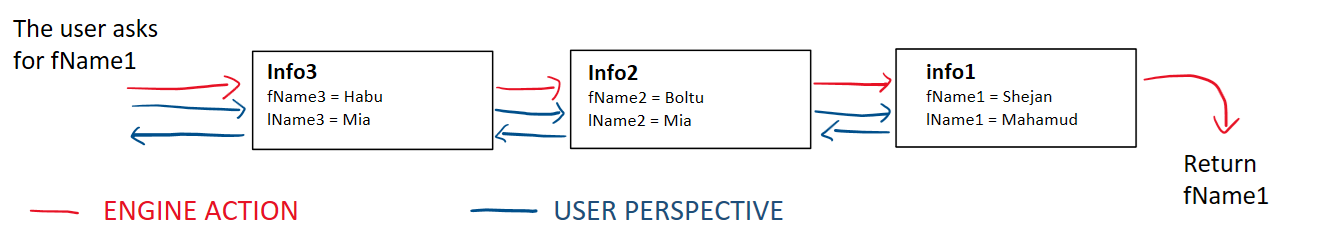
\includegraphics[width=\linewidth]{Images/Prototype chain.png}
    \caption{Prototype chain}
    \label{fig:prototype_chain}
\end{figure}

The example is illustrated in figure \ref{fig:prototype_chain}. When \texttt{info3.fName1} is requested, JavaScript checks \texttt{info3} (not found), then its prototype \texttt{info2} (not found), and finally \texttt{info2}'s prototype \texttt{info1}, where \texttt{fName1} is successfully located. At this point we have to distinguish the actions of the engine from what happens according to the user perspective. When the engine finds \texttt{fName1}, it can simply return it to the user without passing this value back in the chain so that \texttt{info3} can return it. To the eyes of the user, instead, it seems like \texttt{info3} has the requested property so the user thinks that they are communicating only with \texttt{info3} who has all the information contained in the prototype chain.

\section{The Mystery of Primitives}

This lookup mechanism also explains a common JavaScript "mystery": how primitive types like strings and numbers can have methods. This is possible through a process called \textbf{"auto-boxing"} or \textbf{"wrapper objects"}. When you try to access a method on a primitive, like \texttt{name.toLowerCase()}, JavaScript performs these steps behind the scenes:

\begin{enumerate}
    \item
    It temporarily wraps the primitive value in a corresponding object (e.g., \texttt{new String("value")}).
    
    \item
    This temporary object's \texttt{\_\_proto\_\_} points to the appropriate prototype (\texttt{String.prototype}, \texttt{Number.prototype}, etc.).
    
    \item
    The method is found on the prototype and executed.
    
    \item
    The temporary wrapper object is discarded, and the value returns to being a simple primitive.
\end{enumerate}

This elegant system is why it's often said that "everything in JavaScript behaves like an object," even when that's not technically true. Now that we understand the theory of the prototype chain, let's turn to the practical methods used to create and manage these inheritance relationships.

\chapter{Practical Implementation: Creating and Linking Objects}

This section serves as a practical guide to the two primary built-in methods for establishing relationships between objects: \texttt{Object.create()} and \texttt{Object.assign()}. These methods provide developers with direct control over how objects are linked or copied. Choosing the correct method is essential and depends entirely on whether the goal is to establish a dynamic, ongoing delegation or to create a static, one-time copy of an object's properties.

\section{Delegation via Object.create()}

The \texttt{Object.create()} method's core function is to create a new, empty object and set its internal \texttt{\_\_proto\_\_} reference to an existing object passed as an argument. \\

This method establishes a "live" reference, a form of \textbf{delegation}, not a copy. The new object is a lightweight shell that delegates property lookups to its prototype. Any changes made to the prototype object will be immediately reflected in all objects that inherit from it. \\

This behavior is illustrated in the following example. When \texttt{A.a} is modified, the change is visible through \texttt{B} because \texttt{B} is merely pointing to \texttt{A} as its prototype.

\begin{lstlisting}
    var A = {a: 10};
    
    // B is created with A as its prototype
    var B = Object.create(A);
    
    console.log("B.a is: " + B.a); // 10
    
    // Modifying the prototype object A
    A.a = 20;
    
    // The change is reflected in B through the prototype chain
    console.log("B.a after changing A.a is: " + B.a); // 20
\end{lstlisting}

The key advantage of this delegation-based approach is \textbf{memory efficiency}. If the prototype is a "heavyweight" object with many properties, \texttt{Object.create()} allows you to create new objects that inherit its functionality without duplicating all of that data in memory. The new object is just a lightweight reference.

\section{Copying via \texttt{Object.assign()}}

In contrast, the \texttt{Object.assign()} method's purpose is to copy all enumerable own properties from one or more source objects directly onto a target object. \\

This operation creates a \textbf{shallow copy} of the source's properties, effectively breaking the live prototype link. The target object receives its own copies of the source's properties at the time of the assignment. Subsequent changes to the source object will \textit{not} affect the target. \\

The following example demonstrates this detached relationship. After \texttt{B} is created as a copy of \texttt{A}, changing \texttt{A.a} has no effect on \texttt{B.a}.

\begin{lstlisting}
    var A = {a: 20};
    
    // B is created by copying properties from A into a new empty object
    var B = Object.assign({}, A);
    
    console.log("B.a is: " + B.a); // 20
    
    // Modifying the original object A
    A.a = 15;
    
    // B remains unchanged because it is a separate copy
    console.log("A.a after change is: " + A.a); // 15
    console.log("B.a is still: " + B.a); // 20
\end{lstlisting}

\textbf{Warning for Deep Cloning} It is important to note that \texttt{Object.assign()} performs a \textit{shallow} copy. If a source property's value is a reference to another object, only the reference is copied, not the object itself. Both the original and the copy will point to the same nested object.

\section{Comparative Analysis: create vs. assign}

The choice between these two methods depends on the desired relationship between the objects.

\begin{center}
    \begin{tabular}{|p{0.2\linewidth}|p{0.35\linewidth}|p{0.35\linewidth}|}
    \hline
    
        Feature & \texttt{Object.create()} & \texttt{Object.assign()} \\ \hline
        
        \textbf{Core Purpose} & Creates a new object using an existing object as its prototype. & Copies enumerable own properties from source(s) to a target object. \\ \hline
        
        \textbf{Relationship Created} & \textbf{Ongoing lookup-time delegation}. Changes to the prototype are reflected. & \textbf{One-time property copying}. Creates a detached snapshot of properties. \\ \hline
        
        \textbf{Memory Impact} & High efficiency; creates a lightweight reference to the prototype. & Lower efficiency; duplicates properties, consuming more memory for large objects. \\ \hline
        
        \textbf{Primary Use Case} & Implementing prototypal inheritance and sharing functionality. & Merging multiple objects or creating a static snapshot of an object. \\ \hline
    \end{tabular}
\end{center}

Understanding how to create and link objects sets the stage for examining the more nuanced behaviors that can arise within these prototypal structures, such as how JavaScript determines the execution context.

\section{Interaction between the this keyword and the prototype chain}

The value of the \texttt{this} keyword is a frequent point of confusion, but its behavior follows a simple rule: its value is determined by the object that \textit{calls} the function at execution time, not by where the function is defined. It refers to the context of the call. \\

This principle is clearly illustrated in the following example, where the \texttt{bar} object inherits the \texttt{show} method from its prototype, \texttt{foo}.

\begin{lstlisting}
    var foo = {
        message: "Hello",
        show() {
            console.log(this.message);
        }
    };
    
    var bar = {
        message: "World",
        __proto__: foo
    };
    
    bar.show(); // Prints "World"
\end{lstlisting}

Although the \texttt{show} method is defined within the \texttt{foo} object, it is called on the \texttt{bar} object (\texttt{bar.show()}). Therefore, the context for \texttt{this} inside the function becomes \texttt{bar}. When \texttt{this.message} is accessed, it resolves to the \texttt{message} property on \texttt{bar}, which is "World". The \texttt{message} property on \texttt{foo} is effectively \textbf{shadowed}, demonstrating that the call-site, not the definition-site, determines the context.

\chapter{The Compiler's First Pass: Hoisting}

Hoisting is JavaScript's behavior of processing variable and function declarations before any part of the code is executed. During an initial pass, the JavaScript interpreter allocates memory for all declarations, effectively moving them to the top of their scope. However, the way it treats functions and variables differs significantly.

\begin{itemize}
    \item
    \textbf{Functions:} The \textit{entire function declaration} (both the name and the body) is hoisted. This allows a function to be called before it physically appears in the code.
    
    \item
    \textbf{Variables (}\texttt{\textbf{var}}\textbf{):} Only the \textit{declaration} (\texttt{var varA;}) is hoisted, not the assignment (\texttt{= "Hello"}). This means the variable exists from the top of its scope, but its value will be \texttt{undefined} until the line where it is assigned is reached during execution.

    \item
    \textbf{Variables (}\texttt{\textbf{let}} \textbf{and} \texttt{\textbf{const}}\textbf{):} These declarations are also hoisted, but they behave differently. Instead of being initialized with \texttt{undefined}, they are placed in a special state called the \textbf{Temporal Dead Zone (TDZ)} from the start of the scope until their declaration is evaluated.
\end{itemize}

\section{The Temporal Dead Zone (TDZ)}

The \textbf{Temporal Dead Zone} is the time between entering a scope and the actual declaration of a variable declared with \texttt{let} or \texttt{const}. During this period, the variable exists but cannot be accessed.

Attempting to use it results in a \texttt{ReferenceError}.

\begin{lstlisting}
    // Example: Accessing a let variable in TDZ
    function test() {
        console.log(a);
        let a = 10;
    }

    test(); // ReferenceError: Cannot access 'a' before initialization
\end{lstlisting}

This behavior contrasts with \texttt{var}, which would return \texttt{undefined} instead of throwing an error.

\section{Examples: comparing \texttt{var}, \texttt{let}, and \texttt{const}}

\begin{lstlisting}
    // Example 1: Variable not declared at all
    function printVar() {
        console.log(varA);
    }
    printVar(); // ReferenceError: varA is not defined
\end{lstlisting}

\begin{lstlisting}
    // Example 2: var hoisting
    function printVar() {
        console.log(varA); // varA exists but is undefined
        var varA = "Hello";
    }
    printVar(); // undefined
\end{lstlisting}

\begin{lstlisting}
    // Example 3: let in TDZ
    function printLet() {
        console.log(varB);
        let varB = "Hello";
    }
    printLet(); // ReferenceError
\end{lstlisting}

\begin{lstlisting}
    // Example 4: const in TDZ
    function printConst() {
        console.log(varC);
        const varC = "Hello";
    }
    printConst(); // ReferenceError
\end{lstlisting}

\begin{lstlisting}
    // Example 5: Correct usage of let
    function test() {
        let x = 5;
        console.log(x); // 5
    }
    test();
\end{lstlisting}

\begin{lstlisting}
    // Example 6: const must be initialized
    const value = 10; // OK
    const anotherValue; // SyntaxError
\end{lstlisting}

\section{Why TDZ Exists}

The Temporal Dead Zone was introduced to:
\begin{itemize}
    \item prevent accidental use of variables before initialization
    \item make code more predictable
    \item avoid subtle bugs caused by \texttt{undefined} values
\end{itemize}

\section{Two-Pass Execution Model}

The underlying reason for this behavior is that JavaScript works in a \textbf{two-pass way}. In the first pass, it scans the code and allocates memory for all declarations. In the second pass, it executes the code line by line.

\begin{itemize}
    \item \texttt{var}: initialized during the first pass
    \item \texttt{let}/\texttt{const}: created during the first pass but initialized only during execution
\end{itemize}

This distinction explains why accessing \texttt{var} yields \texttt{undefined}, while accessing \texttt{let} or \texttt{const} before initialization results in an error.\\

With a firm grasp of these underlying mechanics, we can now appreciate the modern syntax that was introduced to abstract them away and provide a more predictable development experience.

\chapter{Modern Abstraction: ES6 Classes as Syntactic Sugar}

With the introduction of ECMAScript 6 (ES6), JavaScript received a modern, cleaner syntax for implementing object-oriented patterns: the \texttt{class}. While this syntax provides a more familiar structure for developers coming from class-based languages, it is crucial to understand that it is \textbf{syntactic sugar}. Under the hood, ES6 classes are built directly on top of JavaScript's existing prototypal inheritance system. \\

The following example demonstrates the modern class syntax for creating a \texttt{User}:

\begin{lstlisting}
    class User {
      constructor(name) {
        this.name = name;
      }
      sayHi() {
        console.log(`Hi, I'm ${this.name}`);
      }
    }
    
    const user1 = new User("Charlie");
    user1.sayHi(); // "Hi, I'm Charlie"
\end{lstlisting}

\section{Deconstructing "Syntactic Sugar"}

The term "syntactic sugar" means that the \texttt{class} keyword does not introduce a new object-oriented inheritance model. Instead, it provides a simpler way to work with prototypes. Internally:

\begin{itemize}
    \item
    A \texttt{class} is still a special kind of \textbf{function}.
    
    \item
    Methods defined within the class (like \texttt{sayHi}) are automatically added to the class's \texttt{prototype} property.
    
    \item
    Creating an instance with the \texttt{new} keyword sets the instance's \texttt{\_\_proto\_\_} to the class's \texttt{prototype}, just as it does with a constructor function.
\end{itemize}

We can prove this underlying connection by inspecting the \texttt{User} class and its instance:

\begin{lstlisting}
    // A class is just a function
    console.log(typeof User); // "function"
    
    // The instance's __proto__ points to the class's prototype, establishing the chain
    console.log(user1.__proto__ === User.prototype); // true
\end{lstlisting}

These checks confirm that the class syntax is a powerful abstraction that ultimately resolves to the same prototypal mechanics we have explored. \\

In summary, while the modern \texttt{class} syntax simplifies object creation and inheritance, a deep understanding of the underlying prototype chain remains fundamental to becoming a proficient JavaScript developer. The prototype is the engine of JavaScript's object model, and recognizing its role—even when abstracted by modern syntax—is the key to unlocking the language's full potential.

\chapter{The Core Execution Engine: How JavaScript Runs Code}

To write predictable and efficient code, it is crucial to understand the fundamental components of the JavaScript runtime—the engine, the heap, and the call stack. While modern JavaScript engines employ sophisticated optimizations, a clear mental model of the core execution process remains indispensable. This section deconstructs what happens "under the hood" when a script is executed, revealing the mechanics that govern everything from variable access to function invocation.

\section{The JavaScript Runtime Environment}

The execution of JavaScript code is a collaboration between two key pieces of software: the \textbf{JavaScript Engine} and the \textbf{Host Environment}.

\begin{itemize}
    \item
    The \textbf{JavaScript Engine} is the core component that implements the language, taking source code, parsing it, and executing it. It manages memory and the flow of control.
    
    \item
    The \textbf{Host Environment} provides the context in which the engine runs. Environments like a web browser or Node.js offer external, environment-specific APIs that allow JavaScript to interact with the outside world, such as accessing the HTML DOM, making network requests (\texttt{fetch}), or accessing the file system.
\end{itemize}

\section{Memory Management: The Heap and The Call Stack}

To manage a running program, any language runtime must answer two fundamental questions: "Where do I store my data?" and "What am I currently doing?". In JavaScript, the answers are the Heap and the Call Stack, respectively. JavaScript's memory model is organized into these two primary structures that serve distinct purposes.

\begin{itemize}
    \item
    \textbf{The Heap:} The heap is a large, unstructured region of memory used for dynamic allocation. When you create objects or define variables in your program, they are stored in the heap. This memory is managed automatically by the JavaScript engine's garbage collector, which frees developers from the need to manually allocate and deallocate memory, as is common in languages like C or C++.
    
    \item
    \textbf{The Call Stack:} The Call Stack is a LIFO (Last-In-First-Out) data structure that the JavaScript engine uses to track function execution. When a function is called, a new stack frame, also known as an \textbf{Execution Context}, is created and pushed onto the top of the stack. This frame contains information about the function's arguments and local variables. When the function completes its execution and returns, its frame is popped off the stack. JavaScript is inherently single-threaded, which means it has only one call stack and can therefore only execute one operation at a time.
\end{itemize}

\section{The Execution Context (EC) and Hoisting}

The JavaScript engine executes code by creating an \textbf{Execution Context (EC)}. Each script (global code) and each function invocation generates a new execution context. The creation of an execution context happens in two distinct phases.

\subsection{Global Execution Context}

Before execution begins, the engine creates the \textbf{Global Execution Context (GEC)}. During its creation:

\begin{itemize}
    \item A \textbf{global object} is created (\texttt{window} in browsers)
    \item All global variables and functions become properties of this object
    \item The keyword \textbf{\texttt{this}} is bound to the global object
    \item Memory is allocated for variables and function declarations
\end{itemize}

The global object also acts as a container for Web APIs such as \texttt{setTimeout}, \texttt{XMLHttpRequest}, \texttt{location}, and \texttt{history}.

\subsection{Two Phases of Execution Context Creation}

\begin{enumerate}
    \item
    \textbf{Memory Creation Phase (Hoisting Phase):}  
    During this phase, the engine scans the code without executing it.

    \begin{itemize}
        \item \textbf{Function declarations:} The engine stores a \textbf{reference to the entire function} (including its body)
        \item \textbf{\texttt{var} variables:} Initialized with \texttt{undefined}
        \item \textbf{\texttt{let} and \texttt{const}:} Allocated but left uninitialized (Temporal Dead Zone)
    \end{itemize}

    \textbf{Important:}
    \begin{itemize}
        \item No code is executed in this phase
        \item No function execution contexts are created yet
        \item Only bindings (name → value/reference) are established
    \end{itemize}

    \item
    \textbf{Execution Phase:}  
    In this phase, the engine executes the code line by line.

    \begin{itemize}
        \item Variables are assigned their actual values
        \item Function declarations are skipped (already in memory)
        \item Function calls trigger the creation of new execution contexts
    \end{itemize}

    When a function is invoked:
    \begin{itemize}
        \item a new \textbf{Function Execution Context} is created;
        \item it is pushed onto the \textbf{call stack};
        \item the memory creation phase runs for that function;
        \item the \texttt{arguments} object is created. It stores the values passed to the function at invocation time and includes a \texttt{length} property indicating how many arguments were actually supplied, rather than how many parameters were declared;
        \item \texttt{this} is bound (typically to the global object in non-strict mode);
        \item the function body is executed.
    \end{itemize}

    Once the function finishes, its execution context is removed from the stack.
\end{enumerate}

\subsection{Internal Structure of an Execution Context}

Each execution context contains:

\begin{itemize}
    \item \textbf{Variable Environment:} stores variables and function references
    \item \textbf{Scope Chain:} used to resolve variable access
    \item \textbf{\texttt{this} binding:} determined at runtime
\end{itemize}

\subsection{Example: Memory creation phase and execution phase of a simple print function}

Let us say that we have the simple following function that prints the string "Hello":

\begin{lstlisting}
    printMessage();
    
    function printMessage(){
        var message = "Hello";
        console.log(message);
    }
\end{lstlisting}

\begin{figure}
    \centering
    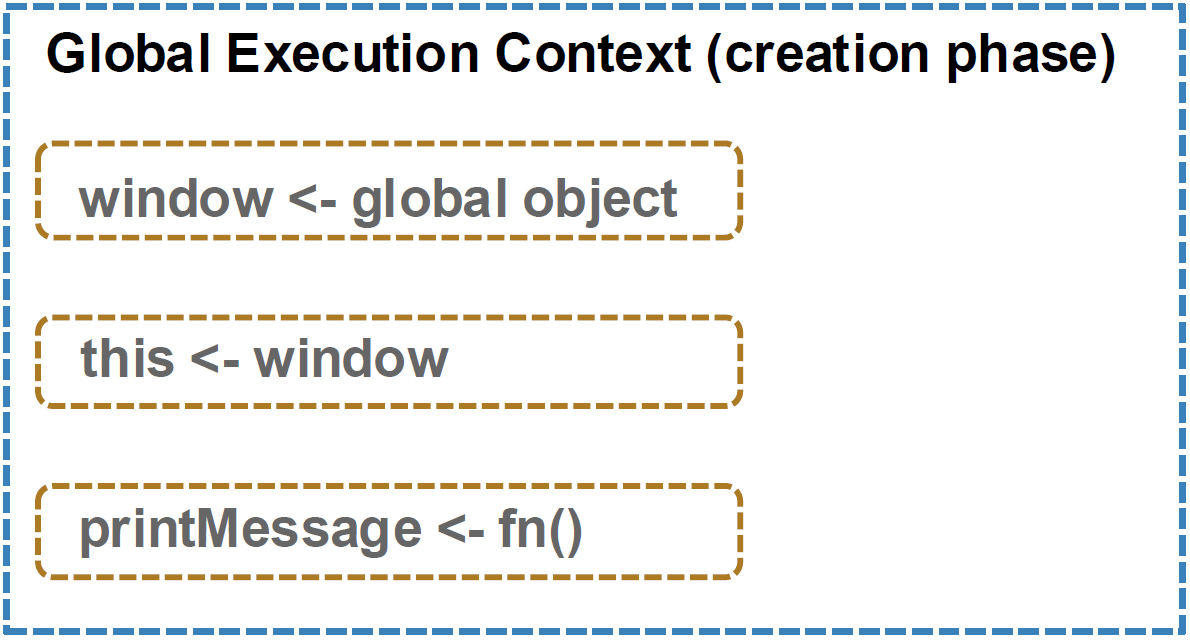
\includegraphics[width=0.5\linewidth]{Images/Function execution 1.png}
    \caption{Creation of the Global Execution Context}
    \label{fig:gec_creation}
\end{figure}

\begin{figure}
    \centering
    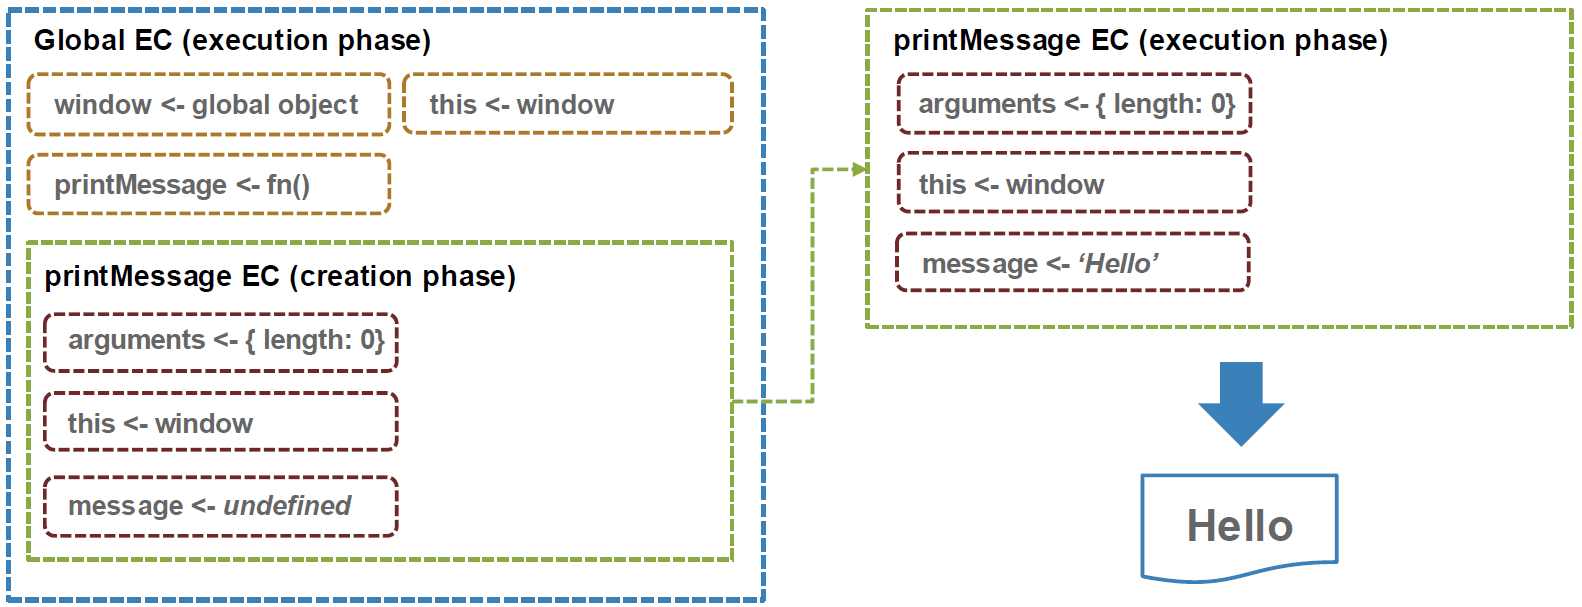
\includegraphics[width=\linewidth]{Images/Function execution 2.png}
    \caption{Creation of the function execution context and execution phase}
    \label{fig:execution_phase}
\end{figure}

The JavaScript engine runs this code in the following steps:

\begin{enumerate}
    \item
    \textbf{Creation of the Global Execution Context} (see figure \ref{fig:gec_creation}):
    \begin{itemize}
        \item The global object is bound to the window
        \item The window is bound to the \texttt{this} keyword
        \item The engine creates a function reference to the \texttt{printMessage} function
    \end{itemize}

    \item
    \textbf{Creation of the printMessage Execution Context} (see figure \ref{fig:execution_phase}):
    \begin{itemize}
        \item The \texttt{arguments} object is created and contains the arguments passed to the function (in this case, \texttt{length = 0})
        \item The window is bound to the \texttt{this} keyword
        \item The JavaScript engine binds the \texttt{message} variable to the value \texttt{undefined}
    \end{itemize}

    \item
    \textbf{Execution phase of the printMessage function}
    \begin{enumerate}[label=(\arabic*)]
        \item The engine assigns the value to the \texttt{message} variable
        \item The engine prints the variable
    \end{enumerate}
\end{enumerate}

\subsection{Visual Model}

The following diagram illustrates the difference between the memory phase and the execution phase:

\begin{center}
    \begin{tabular}{|c|c|}
        \hline
        \textbf{Memory Creation Phase} & \textbf{Execution Phase} \\
        \hline
        Global EC created & Code executed line by line \\
        \hline
        \texttt{var x → undefined} & \texttt{x = 10} \\
        \hline
        \texttt{let y → TDZ} & \texttt{y = 20} \\
        \hline
        \texttt{foo → function reference} & \texttt{foo()} called → new EC created \\
        \hline
    \end{tabular}
\end{center}

\subsection{Call Stack Behavior}

Let us make an example of nested function call and illustrate what happens in the stack.

\begin{lstlisting}
    function bar(){
        ...
    }

    function foo(){
        ...
        bar();
        ...
    }

    // Call of the foo function from the Global EC
    foo();
\end{lstlisting}

\begin{figure}
    \centering

    \begin{tikzpicture}
        % Dimensioni
        \def\w{6}      % larghezza
        \def\h{0.8}    % altezza di ogni blocco
        
        % Coordinate base
        \coordinate (bottom) at (0,0);
        
        % Disegno dei rettangoli (dal basso verso l'alto)
        \draw (0,0) rectangle (\w,\h) node[pos=.5]{\texttt{Global EC}};
        \draw (0,\h) rectangle (\w,2*\h) node[pos=.5]{\texttt{foo EC} (after function call)};
        \draw (0,2*\h) rectangle (\w,3*\h) node[pos=.5]{\texttt{bar EC} (nested call)};
        
        % Titolo
        \node at (\w/2,3*\h + 1.2) {\textbf{Call Stack}};
        
        % Puntini verticali sopra lo stack
        \node at (\w/2,3*\h + 0.2) {$\cdot$};
        \node at (\w/2,3*\h + 0.4) {$\cdot$};
        \node at (\w/2,3*\h + 0.6) {$\cdot$};
    
    \end{tikzpicture}
    
    \caption{Stack behavior during a nested function call}
    \label{fig:stack_nested_call}
\end{figure}

Execution contexts are pushed onto the stack when functions are invoked and popped when they return. In fact, in figure \ref{fig:stack_nested_call} we can see that at the bottom of the stack we have the global EC. Then, when the function \texttt{foo} is invoked, its EC is put on top of the global one. When the function \texttt{foo} invokes the function \texttt{bar}, the context of the latter is put on top of the stack.

\subsection{Key Observations}

\begin{itemize}
    \item Hoisting does \textbf{not} execute functions
    \item Functions are stored as \textbf{references}, not as execution contexts
    \item Execution contexts are created \textbf{only when functions are invoked}
    \item The call stack keeps track of the execution order
\end{itemize}

\begin{quote}
    \centering
    \textit{JavaScript first prepares the environment (memory phase), then executes the code (execution phase).}
\end{quote}

This synchronous, single-threaded execution model is straightforward but presents a significant challenge: how can JavaScript handle time-consuming operations without freezing the entire application?

\chapter{The Concurrency Model: Event Loop and Queues}

\begin{figure}
    \centering
    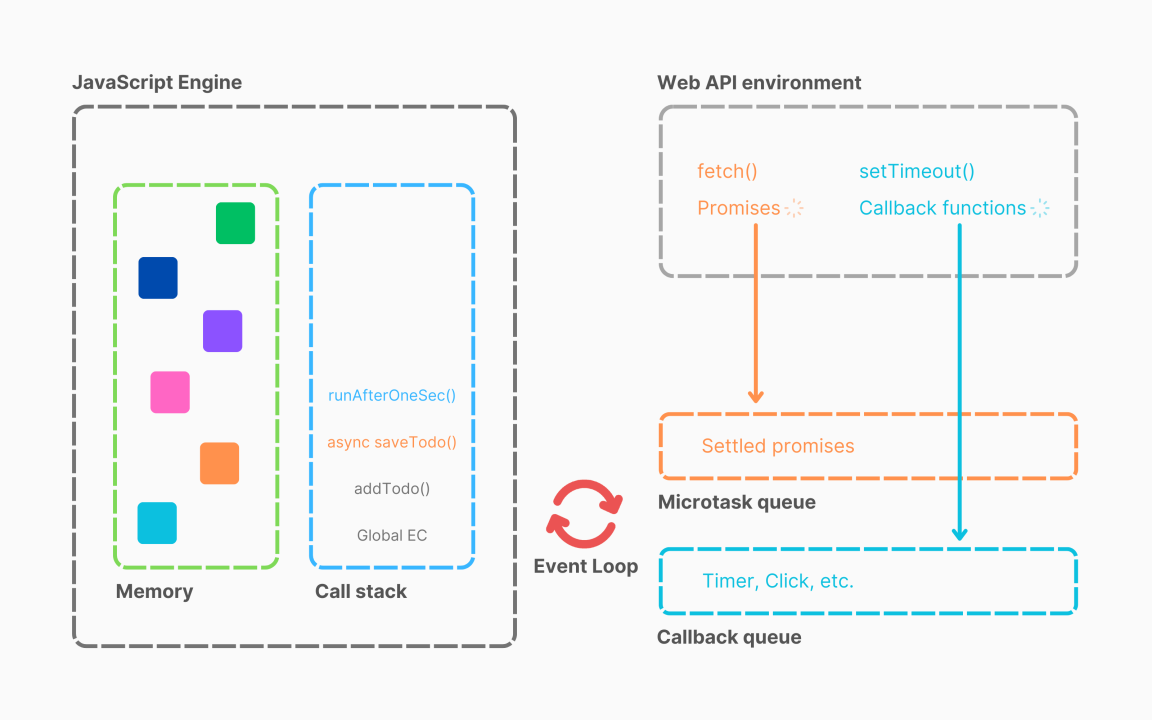
\includegraphics[width=\linewidth]{Images/JS_runtime_environment.png}
    \caption{JavaScript runtime environment}
    \label{fig:js_runtime_environment}
\end{figure}

JavaScript's concurrency model is the architectural answer to the limitations of its single-threaded nature. Despite having only one call stack, JavaScript masterfully handles asynchronous operations like network requests or timers without blocking the main thread. This non-blocking behavior is not magic; it is achieved through a sophisticated interplay between the JavaScript engine, APIs provided by the host environment, an Event Loop, and a set of distinct job queues (see figure \ref{fig:js_runtime_environment}).

\section{The Problem with a Single Thread}

The limitation of a single call stack is that if a long-running synchronous function is executing, the entire program is blocked. In a browser environment, this means the web page becomes unresponsive; it cannot process user interactions like clicks or scrolls, nor can it render any updates. This is precisely why JavaScript \texttt{<script>} tags are often placed at the end of an HTML document's \texttt{<body>}—it allows the browser to render the page content first before executing potentially blocking scripts.

\section{The Components of Asynchronous Execution}

To enable non-blocking behavior, the JavaScript runtime environment includes several components that work in concert with the engine.

\begin{itemize}
    \item
    \textbf{Web APIs / Host Environment APIs:} Asynchronous operations are not handled by the JavaScript engine itself. Instead, they are offloaded to APIs provided by the host environment (e.g., the browser or Node.js). Operations like \texttt{setTimeout}, DOM events, and \texttt{fetch} requests are managed by these external APIs. When an operation completes, its associated callback function is prepared for execution.
    
    \item
    \textbf{The Macrotask Queue (or Callback Queue):} This is a FIFO (First-In-First-Out) queue where callbacks for completed asynchronous tasks are placed. For example, when a \texttt{setTimeout} timer expires or a user clicks a button, its callback function is added to this queue.
    
    \item
    \textbf{The Microtask Queue:} This is a high-priority FIFO queue where callbacks for promises (e.g., \texttt{.then()}, \texttt{.catch()}) and \texttt{async/await} are placed. Microtasks are always processed before any tasks from the Macrotask Queue.
    
    \item
    \textbf{The Event Loop:} The Event Loop is the central coordinator. Its primary role is to continuously monitor the Call Stack and the two queues. When the Call Stack is empty, the Event Loop checks the queues and moves tasks to the stack for execution according to a strict order of priority.
\end{itemize}

\section{The Order of Operations}

The event loop manages the precise order of execution with a strict set of rules, ensuring a predictable and non-blocking flow.

\begin{enumerate}
    \item
    Execute all synchronous code currently on the Call Stack until it is empty.
    
    \item
    Check the Microtask Queue. If it has tasks, execute all of them in order until the Microtask Queue is empty.
    
    \item
    Check the Macrotask Queue. If it has a task, take the first one, push its callback to the Call Stack, and execute it.
    
    \item
    Repeat the cycle. After the single macrotask completes and the Call Stack is empty again, the Event Loop returns to step 2, always completely draining the Microtask Queue before checking for the next macrotask.
\end{enumerate}

\paragraph{Starvation of macrotasks}
Although this scheduling model ensures determinism, it may lead to starvation. If microtasks continuously enqueue new microtasks, the Microtask Queue may never become empty. As a result, macrotasks (e.g., \texttt{setTimeout}) may be indefinitely delayed. This behavior is not a flaw but a consequence of the design choice that gives strict priority to microtasks.\\

\section{Example of synchronous code execution}

\begin{figure}
    \centering
    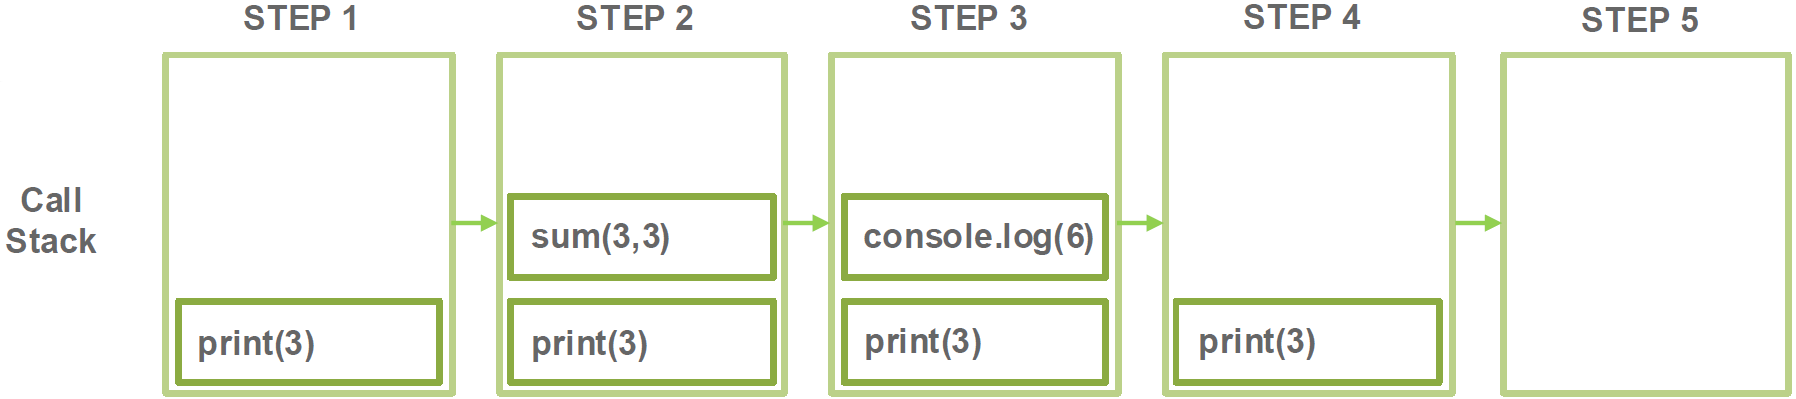
\includegraphics[width=\linewidth]{Images/Syncronous code execution cut.png}
    \caption{Synchronous code execution}
    \label{fig:synchronous_code_execution}
\end{figure}

Let us expose how the JavaScript runtime environment executes the following code.

\begin{lstlisting}
    function sum(x,y){
        return x + y;
    }
    
    function print(x){
        var tot = sum(x,x);
        console.log(tot);
    }
    
    print(3);
\end{lstlisting}

This code only contains synchronous functions so, the JavaScript engine will only employ the call stack as depicted in figure \ref{fig:synchronous_code_execution}.\\

The way the call stack works is simple:
\begin{itemize}
    \item It is initially empty
    \item When a function is invoked, a stack frame is pushed on top of the stack
    \item When a function is completed, a stack frame is popped from the top of the stack
\end{itemize}

In this example, the first invoked function is \texttt{print(3)}. It is pushed onto the call stack with the evaluated argument value \texttt{3}. The newly created execution context of the function \texttt{print(3)} has a dedicated memory space called the \textbf{variable environment} (or lexical environment, more on this topic in the following chapters). The variable environment contains the following bindings:
\begin{itemize}
    \item $x \leftarrow 3$
    \item $tot \leftarrow undefined$
\end{itemize}

When the body of the \texttt{print(3)} function invokes the function \texttt{sum(x,x)} it first resolves the value of \texttt{x} (which is $3$) from the current execution context and then pushes the instantiated invocation \texttt{sum(3,3)} onto the stack. The lexical scope of the \texttt{sum(3,3)} function contains the following associations:
\begin{itemize}
    \item $x \leftarrow 3$
    \item $y \leftarrow 3$
\end{itemize}

The execution of the \texttt{sum(3,3)} function returns the value $6$ which is associated to the variable \texttt{tot}. So, now the lexical scope of the \texttt{print(3)} function contains the following associations:
\begin{itemize}
    \item $x \leftarrow 3$
    \item $tot \leftarrow 6$
\end{itemize}

Now, the body of the \texttt{print(3)} function invokes \texttt{console.log(6)}, printing the value to the console. Although \texttt{console.log} is a host function provided by the environment (e.g., the browser or Node.js), its invocation still creates a JavaScript execution context and is managed through the call stack. However, its internal implementation is not executed by the JavaScript engine itself, but is delegated to the host environment.\\

This execution model also applies to Web APIs such as \texttt{setTimeout}, \texttt{fetch}, and DOM-related functions. The JavaScript engine handles their invocation, but the actual operations (timers, network requests, DOM manipulation) are executed by the host environment. Once completed, their callbacks are placed into the appropriate task queue (e.g., callback queue or microtask queue) to be processed later by the event loop.\\

Finally, the value $6$ is printed in the console, the execution context of the \texttt{console.log(6)} function is popped from the stack, the body of the \texttt{print(3)} function ends and the execution context of the latter is popped from the stack.\\

Consider that while the call stack is executing synchronous code, the browser cannot perform other tasks, which may lead to blocking behavior and this create concurrency problems. We don't notice this interruption for short task handled using the call stack. For longer tasks, instead, the JavaScript runtime uses the callback queue and the event loop to handle asynchronous operations. The following example exposes an example of callback queue usage.

\section{Example of asynchronous code execution}

\begin{figure}
    \centering
    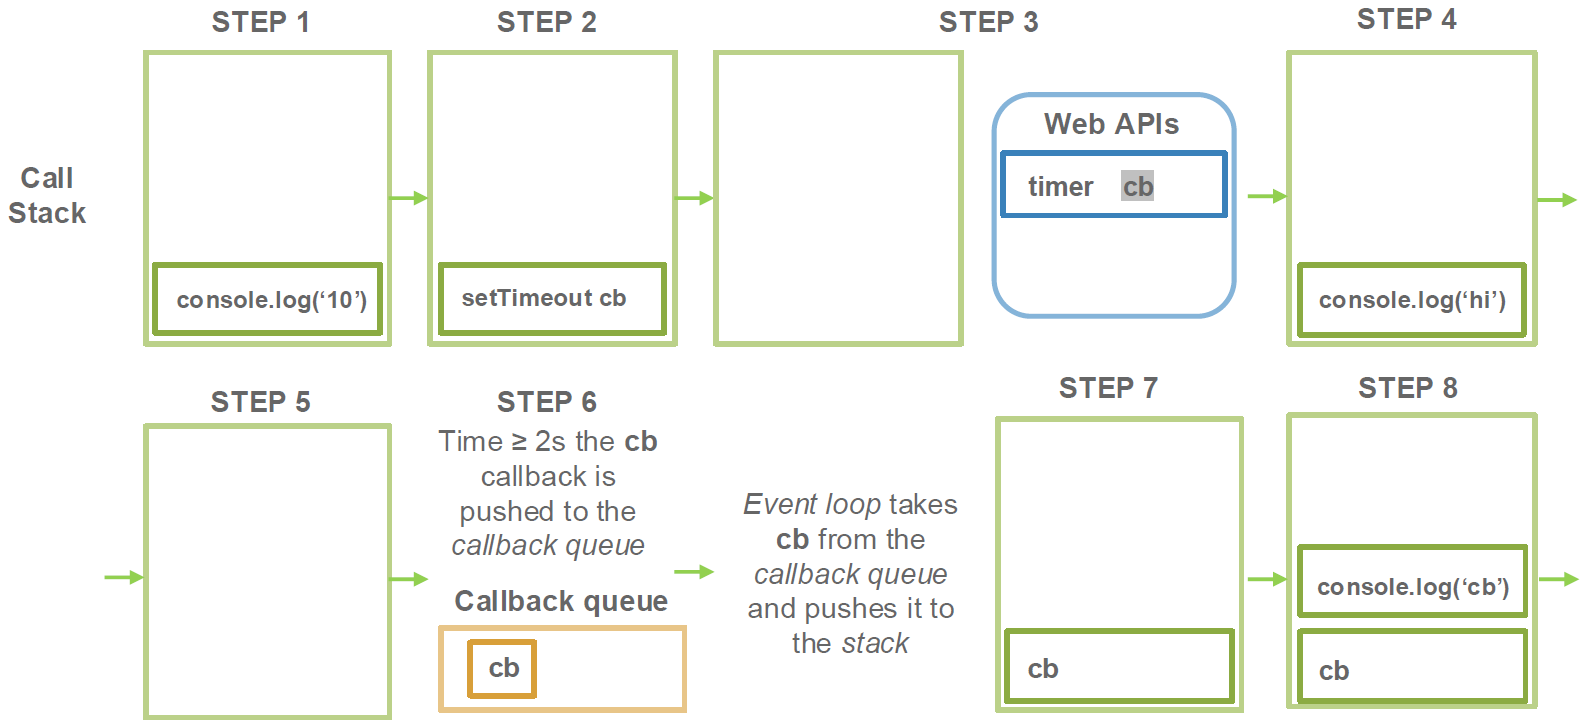
\includegraphics[width=\linewidth]{Images/Macrotask execution.png}
    \caption{Example of macrotask execution}
    \label{fig:macrotask_execution}
\end{figure}

Figure \ref{fig:macrotask_execution} shows an example of macrotask execution. The key idea is that a function executed in the call stack can delegate work to a Web API, which later schedules a callback in the callback queue (macrotask queue).\\

It is important to note that when the call stack becomes empty, the event loop first processes all pending microtasks (if any), and only then takes one macrotask from the callback queue and pushes it onto the call stack for execution.\\

Let us analyze the following code step by step:

\begin{lstlisting}
    console.log('10');
    
    setTimeout(function cb() {
        console.log('cb');
    }, 2000);
    
    console.log('hi');
\end{lstlisting}

\begin{enumerate}
    \item The global execution context starts executing the code.

    \item \texttt{console.log('10')} is pushed onto the call stack, executed, and then removed. The value \texttt{10} is printed to the console.

    \item \texttt{setTimeout(...)} is pushed onto the call stack and executed. The JavaScript engine delegates the timer operation to the Web API environment, passing the callback function \texttt{cb} and the delay (2000 ms). The \texttt{setTimeout} call then completes and is removed from the call stack.

    \item While the timer is running in the Web API environment, the JavaScript engine continues executing the remaining synchronous code.

    \item \texttt{console.log('hi')} is pushed onto the call stack, executed, and then removed. The value \texttt{hi} is printed to the console.

    \item After approximately 2000 ms, the Web API finishes the timer and places the callback function \texttt{cb} into the callback queue (macrotask queue).

    \item When the call stack becomes empty, the event loop checks the microtask queue and processes all its tasks (if any). Since there are no microtasks in this example, it proceeds to the macrotask queue.

    \item The event loop takes the callback \texttt{cb} from the macrotask queue and pushes it onto the call stack.

    \item The callback function \texttt{cb} is executed, printing \texttt{'cb'} to the console, and then removed from the call stack.
\end{enumerate}

This execution model allows JavaScript to remain non-blocking: long-running or delayed operations are handled outside the main thread, while the event loop ensures their callbacks are executed at the appropriate time.\\

The JavaScript runtime environment is an elegant system that allows JavaScript to remain responsive while handling complex asynchronous flows. The primary tools developers use to manage the state and scope of these asynchronous callbacks are closures and promises.

\chapter{Managing Scope and State: Closures}

The concept of scope is fundamental to managing variable accessibility and preventing unintended side effects in a program. JavaScript employs lexical scoping, which determines variable access based on where functions and variables are written in the source code. A powerful and essential consequence of this scoping model is the closure, a mechanism that allows functions to maintain access to their surrounding state.

\section{Lexical Scoping}

\textbf{Scope} defines the context that determines where variables and functions are accessible. JavaScript uses \textbf{lexical scoping} (also known as static scoping), meaning the engine determines the scope of variables based on their physical position in the source code, not during execution. A key principle of lexical scoping is that inner scopes have access to variables defined in their outer scopes. This hierarchical structure allows for a clear and predictable organization of code.\\

Let us analyze the following example:
\begin{lstlisting}
    function print(){
      //function scope
      let counter = 0;
      console.log(counter);
    }
    
    print(); // 0
    console.log(counter); // ReferenceError: counter is not defined
\end{lstlisting}

In this case we get a reference error because the we are trying to access the variable \texttt{counter} from an outer scope. We can consider it as an advantage because this allows us to have variables with the same name in different scopes. For instance:
\begin{lstlisting}
    function print(){
      //function scope
      let counter = 0;
      console.log(counter);
    }
    
    print(); // 0
    
    let counter = 10;
    console.log(counter); // 10
\end{lstlisting}

In this case we have two variables named \texttt{counter} and the interpreter does not raise an error because it understands that the counter used in the \texttt{print} function scope refers to the variable initialized with a value of $0$ while the counter used in the outer scope refers to the one initialized with a value $10$.

\section{Defining a Closure}

A \textbf{closure} is a function that is bundled with its surrounding state—the lexical environment. In practical terms, a closure is a nested function that "remembers" the variables from the scope where it was created (the one of the outer function), even if it is executed in an entirely different scope at a later time. This is possible because the inner function maintains a live reference to the \textit{Execution Context} of its parent—specifically, its lexical environment—even after the parent function's EC has been popped from the call stack.

\section{Practical Application of Closures}

Closures are not merely a theoretical concept; they are a powerful tool for creating private state that persists across multiple function calls. Consider the following counter example:

\begin{lstlisting}
    function outerFunction(){
        // Outer scope
        var counter = 0;
        
        function innerFunction(){
            // Inner scope
            console.log(counter);
            counter += 1;
        }
        
        return innerFunction;
    }
    
    const myInnerFunction = outerFunction();
    myInnerFunction(); // 0
    myInnerFunction(); // 1
    myInnerFunction(); // 2
\end{lstlisting}

In this code, \texttt{outerFunction} is invoked, which initializes the \texttt{counter} variable to \texttt{0}. It then returns \texttt{innerFunction}, which is assigned to the constant \texttt{myInnerFunction}. Because \texttt{innerFunction} is a closure, it maintains a persistent reference to the lexical environment where \texttt{counter} lives. Each time \texttt{myInnerFunction} is invoked, it can access and modify this same \texttt{counter} variable. The \texttt{counter} variable is effectively private, as it cannot be accessed from the global scope, yet its state is preserved between calls. \\

Crucially, \texttt{outerFunction} is invoked \textit{only once}. If it were called each time, the \texttt{counter} would be reset to \texttt{0} with every call. By storing the returned \texttt{innerFunction} in \texttt{myInnerFunction}, we preserve the closure's lexical environment, allowing the \texttt{counter} state to persist across multiple calls. \\

This ability to "remember" state is also foundational to how Promises work; the executor function passed to a \texttt{Promise} constructor relies on a closure to access variables from its surrounding context.

\chapter{Asynchronous Operations with Promises}

A \texttt{Promise} is a foundational object in modern JavaScript for managing asynchronous operations. It serves as a proxy for a value that will be available in the future, allowing asynchronous code to be written in a more manageable, readable, and composable way than with traditional callback-based approaches. It represents the eventual completion or failure of an asynchronous task and its resulting value.

\section{The Promise Object and its States}

The \texttt{Promise} object can exist in one of three distinct states:

\begin{itemize}
    \item
    \texttt{pending}: The initial state. The asynchronous operation has not yet completed.
    
    \item
    \texttt{fulfilled}: The operation completed successfully, resulting in a value.
    
    \item
    \texttt{rejected}: The operation failed, resulting in a reason (typically an error object).
\end{itemize}

A promise is considered \textbf{settled} when it is either fulfilled or rejected. Once settled, a promise is immutable and its state cannot change.

\section{Creating and Consuming Promises}

\subsection{Creating a Promise}

A promise is created using the \texttt{new Promise(executor)} constructor. The \texttt{executor} is a function that runs immediately and is passed two arguments: \texttt{resolve} and \texttt{reject}. These are callback functions provided by the JavaScript engine.

\begin{itemize}
    \item
    \texttt{resolve(value)}: Called when the asynchronous operation completes successfully.
    
    \item
    \texttt{reject(reason)}: Called when the operation fails.
\end{itemize}

The executor's role is to initiate an asynchronous operation and call the appropriate callback to settle the promise. Because the executor function cannot be passed custom arguments, it relies on a \textbf{closure} to capture and access variables from its surrounding scope.

\begin{lstlisting}
    var promise = new Promise(function(resolve, reject){
        // let state = "success";
        let state = "network error";
    
        if (state != "success"){
            // The argument of the reject callback is the failure message
            reject("The operation was not successful");
        } else {
            // The argument of the resolve callback is the success message
            resolve("The operation WAS succesful");
        }
    });
\end{lstlisting}

\subsection{Consuming a Promise}

The eventual result of a promise is handled by attaching callbacks using the \texttt{.then()} and \texttt{.catch()} methods. For example, the previously defined promise can be handled as follows:
\begin{lstlisting}
    promise.then(
      function (successMessage){
        console.log(successMessage);
    })
    .catch(
      function (failureMessage){
        console.log(failureMessage);
    });
\end{lstlisting}

\begin{itemize}
    \item
    \texttt{.then(onFulfilled)}: The \texttt{onFulfilled} handler is called when the promise is fulfilled and receives as an argument the data provided in the \texttt{resolve} callback in the promise.
    
    \item
    \texttt{.catch(onRejected)}: The \texttt{onRejected} handler is called when the promise is rejected and receives as an argument the data provided in the \texttt{reject} callback in the promise.
\end{itemize}

Crucially, both \texttt{.then()} and \texttt{.catch()} return a \textbf{new promise}, which is the key to creating clean, sequential asynchronous workflows through chaining.

\section{Promise Chaining and async/await}

\textbf{Promise chaining} is the practice of executing multiple asynchronous operations in sequence. To properly chain promises, it is critical to \textit{\textbf{return}} a value or another promise from within a \texttt{.then()} handler. If a promise is not returned, the next \texttt{.then()} in the chain will execute immediately with a value of \texttt{undefined}, leading to a "floating promise" that cannot be tracked.

\paragraph{Correct promise chaining}

In a correct chain, each \texttt{.then()} returns a value or a new promise:

\begin{lstlisting}
    function step1() {
        return Promise.resolve("Step 1 completed");
    }
    
    function step2(prevResult) {
        return Promise.resolve(prevResult + " -> Step 2 completed");
    }
    
    step1()
    .then(function(result){
        console.log(result);
        return step2(result);
    })
    .then(function(result){
        console.log(result);
    });
\end{lstlisting}

\textbf{Output:}
\begin{lstlisting}
    Step 1 completed
    Step 1 completed -> Step 2 completed
\end{lstlisting}

\paragraph{Floating promise (incorrect chaining)}

If a promise is not returned, the chain breaks:

\begin{lstlisting}
    step1()
    .then(function(result){
        console.log(result);
        step2(result); // NOT returned
    })
    .then(function(result){
        console.log(result); // undefined
    });
\end{lstlisting}

In this case, the second \texttt{.then()} does not wait for \texttt{step2()} to complete, because its promise is not returned. This leads to loss of control over the asynchronous flow.

\paragraph{Using async/await}

Modern JavaScript provides \texttt{\textbf{async/await}}, which is syntactic sugar built on top of promises. It allows asynchronous code to be written in a sequential style.

\begin{lstlisting}
    async function runSteps() {
        let result1 = await step1();
        console.log(result1);
    
        let result2 = await step2(result1);
        console.log(result2);
    }
    
    runSteps();
\end{lstlisting}

\textbf{Important notes:}
\begin{itemize}
    \item \texttt{await} can only be used inside \texttt{async} functions
    \item \texttt{await} pauses the function execution (non-blocking) until the promise is resolved
    \item under the hood, \texttt{async/await} is still based on promises and the microtask queue
\end{itemize}

These foundational patterns enable developers to manage simple asynchronous tasks, but real-world applications often require more sophisticated patterns for handling multiple concurrent operations and complex error scenarios.

\section{Advanced Promise Patterns}

While basic promise chaining is sufficient for many tasks, modern applications often require coordinating multiple asynchronous operations concurrently or implementing sophisticated error recovery logic. Advanced promise patterns and static methods provide the tools needed to manage these complex scenarios gracefully.

\subsection{Concurrent Operations}

The \texttt{Promise} object includes four static methods for handling concurrent operations. Each method takes an iterable of promises and returns a single promise whose behavior depends on the outcomes of the input promises.

\begin{center}
    \begin{tabular}{|p{0.25\linewidth}|p{0.65\linewidth}|} \hline
        Method & Behavior \\ \hline
        
        \texttt{Promise.all()} &
        Fulfills when \textbf{all} of the input promises have fulfilled, with an array of their fulfillment values. It rejects immediately if \textbf{any} of the input promises reject. \\ \hline
        
        \texttt{Promise.allSettled()} &
        Fulfills when \textbf{all} input promises have settled (either fulfilled or rejected), with an array of objects describing the outcome of each promise. \\ \hline
        
        \texttt{Promise.any()} &
        Fulfills as soon as \textbf{any} of the input promises fulfill, with that promise's fulfillment value. It rejects only if \textbf{all} of the input promises reject. \\ \hline
        
        \texttt{Promise.race()} & Settles (fulfills or rejects) as soon as \textbf{any} of the input promises settle, adopting the outcome of that first promise. \\ \hline
    \end{tabular}
\end{center}

\subsection{Advanced Error Handling}

A robust application must handle errors gracefully. Promises offer flexible patterns for error recovery. The standard approach is to place a single \texttt{.catch()} at the end of a promise chain. This acts as a global handler, catching any rejection that occurs in any of the preceding \texttt{.then()} blocks. \\

For more precise error recovery, promise chains can be nested. An inner \texttt{.catch()} handler can catch failures from a specific part of the chain, allowing the program to handle and recover from non-critical failures while still allowing the outer chain to proceed. Critical failures from higher up in the chain will bypass the inner \texttt{catch} and be caught by the final, outer handler. \\

These advanced patterns provide the control flow necessary to build complex, resilient applications, shifting the focus from managing asynchronicity to structuring the code itself.

\section{Example: Call Stack, Microtasks, and Macrotasks}

The following example illustrates how the JavaScript runtime environment coordinates the execution of synchronous code, microtasks (Promises), and macrotasks (Web APIs such as \texttt{setTimeout}).

\begin{lstlisting}
    console.log("Start");
    
    setTimeout(() => {
        console.log("Macrotask (setTimeout)");
    }, 0);
    
    Promise.resolve()
        .then(() => {
            console.log("Microtask 1 (Promise)");
        })
        .then(() => {
            console.log("Microtask 2 (chained Promise)");
        });
    
    console.log("End");
\end{lstlisting}

\subsection{Expected Output}

\begin{lstlisting}
    Start
    End
    Microtask 1 (Promise)
    Microtask 2 (chained Promise)
    Macrotask (setTimeout)
\end{lstlisting}

\subsection{Step-by-Step Execution}

\begin{enumerate}
    \item \textbf{Synchronous Execution (Call Stack)}
    \begin{enumerate}[label*=\arabic*.]
        \item \texttt{console.log("Start")} is pushed to the call stack and executed.
        \item \texttt{setTimeout(...)} is invoked and delegated to the Web APIs environment.
        \item The Promise is resolved immediately, and its \texttt{.then()} callbacks are placed in the \textbf{Microtask Queue}.

        At this point, one might think that between the \texttt{Promise.resolve()} instruction and the \texttt{console.log("End")} instruction the call stack is empty so the JavaScript engine would run the microtasks. Actually not. The JavaScript engine considers as synchronous code all the code in the main script. After the main script finishes it checks for the microtask queue and the macrotask queue so, the right mental model is:\\
        $Main~script\rightarrow [Empty~call~stack]\rightarrow Microtask~queue\rightarrow Macrotask~queue$
        
        \item \texttt{console.log("End")} is executed.
    \end{enumerate}

	The call stack is now empty.
	
    \item \textbf{Microtask Queue Execution}
    \begin{enumerate}[label*=\arabic*.]
        \item The event loop processes the Microtask Queue.
        \item \texttt{"Microtask 1"} is moved from the queue to the call stack and executed.
        \item The chained \texttt{.then()} adds another microtask in the queue. This is moved from the queue to the stack and executed immediately after.
    \end{enumerate}
    
    After all microtasks are completed, the event loop checks the Macrotask Queue.

    \item \textbf{Macrotask Queue Execution}
    \begin{enumerate}[label*=\arabic*.]
        \item The callback from \texttt{setTimeout} is moved to the call stack.
        \item \texttt{"Macrotask (setTimeout)"} is printed.
    \end{enumerate}
\end{enumerate}

\subsection{Key Observations}

\begin{itemize}
    \item Microtasks (Promises) have higher priority than macrotasks.
    \item All microtasks are executed before any macrotask.
    \item Even with a delay of \texttt{0 ms}, \texttt{setTimeout} does not execute immediately.
    \item The event loop ensures that the call stack is empty before processing queued tasks.
\end{itemize}

\chapter{Structuring Code: Object Creation Patterns}

\section{Foundations of Design Patterns in JavaScript}

In the discipline of software architecture, a ``pattern'' is analytically defined as a recurring, high-level solution to a common design problem. These are not proprietary algorithms, but rather structured blueprints that have been distilled from repeated implementations across diverse software systems. The lineage of this conceptual framework traces back to the architect Christopher Alexander's work in urban design and was formally introduced to software engineering by the ``Gang of Four'' (Gamma, Vlissides, Johnson, and Helm) in 1994. In the context of large-scale JavaScript development, patterns are strategic tools used to manage the inherent complexity of a language that lacks the rigid, static structures of traditional class-based environments.\\

Object Creation Patterns are specialized architectural structures designed to handle the complexities of instantiation. Unlike class-based languages that rely on formal ``blueprints,'' JavaScript's prototype-based nature is fundamentally more flexible and ``wild,'' focusing on the relationships between live objects. This flexibility necessitates a disciplined approach to how objects are created and linked. Historically, the evolution of these patterns was driven by a dual strategic requirement: the need for memory efficiency through shared behavior and the demand for robust state encapsulation.

\section{The Object Decorator Pattern}

The Object Decorator---often referred to as a ``Wrapper''---is a structural pattern that evaluates the extension of object functionality at runtime. From an architectural standpoint, it favors aggregation and composition over static inheritance. This allows developers to avoid the ``combinatorial explosion'' of subclasses that occurs when attempting to model every possible variation of a component at design time.\\

A useful analogy for junior developers is that of clothing: a base entity (the person) can wrap themselves in a sweater, then a jacket, and finally a raincoat. Each layer extends the core ``weather resistance'' behavior without altering the underlying person or requiring a new ``RainyWeatherPerson'' subclass. In implementation, a decorator function accepts an existing object and augments it with new properties or methods, often wrapping existing logic to add pre- or post-processing capabilities.\\

This strategy is implemented creating a function that accepts a target object as a parameter, adds properties/methods (wrapping original logic), and returns the augmented instance.

\begin{itemize}
    \item
        \textbf{Pros:}
        \begin{itemize}
            \item Dynamic composition;
            \item Adheres to the Open/Closed Principle;
            \item Avoids subclass bloat;
            \item Allows for runtime behavior modification.
        \end{itemize}

    \item 
        \textbf{Cons:}
        \begin{itemize}
            \item High memory overhead;
            \item Creates significant \textbf{Garbage Collection (GC) pressure} due to unique function objects;
            \item Difficult to track source logic;
            \item Potential for name collisions.
        \end{itemize}

    \item 
        \textbf{Typical Use Cases:}
        \begin{itemize}
            \item Middleware systems (e.g., Express.js);
            \item Dynamic UI feature flags;
            \item Plugin architectures where third-party extension is required.
        \end{itemize}
\end{itemize}

\subsection{Example of decorator pattern usage}

Let us make an example in which we want to turn a generic object into a car. In this case we create a decorator function that takes in input the generic object and add the \texttt{position} property and the \texttt{move} function. Let us make a first example in which we only add the \texttt{position} property and create the \texttt{move} function externally to the decorator function.

\begin{lstlisting}
    var buildcar = function(obj, position){
        obj.position = position;
        return obj;
    };
    
    var move = function(car){
        car.position++;
    };
    
    var carA = buildcar({}, 1);
    move(carA);
\end{lstlisting}

\texttt{buildcar} is our decorator function which takes the object in input, adds the \texttt{position} property and returns the decorated object. In the final part of the snippet we use the decorator function on the empty object (\texttt{\{\}}) and we use the \texttt{move} function on the object returned by the decorator function. The schematization of the first technique is illustrated in figure \ref{fig:decorator_1}.\\

\begin{figure}
    \centering
    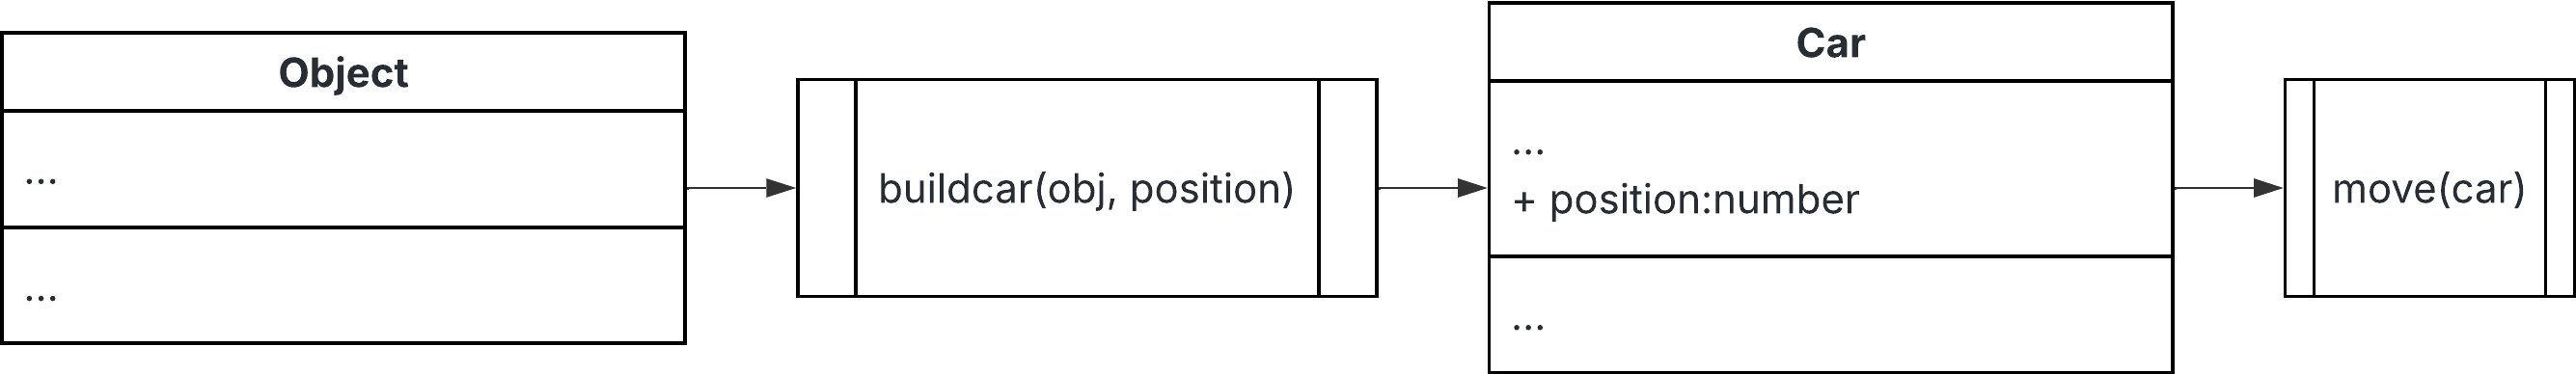
\includegraphics[width=\linewidth]{Images/Decorator 1.png}
    \caption{Example of usage of the decorator function to add only an attribute to an object}
    \label{fig:decorator_1}
\end{figure}

Using an external function is more memory efficient because decorated objects are lighter but it exposes a public function. This may introduce a vulnerability in a context in which we want strong encapsulation and true private state. For this reason, the decorator pattern also allows us to add functions to objects. In the following example we use this other technique.

\begin{lstlisting}
    var buildcar = function(obj, position){
        obj.position = position;
        obj.move = function(){
            // obj always refers to the same object
            obj.position++;
        }
        return obj;
    };
    
    var carA = buildcar({}, 1);
    carA.move();
\end{lstlisting}

In this case, the \texttt{buildcar} function creates a closure scope and the \texttt{obj} variable inside the function will always point to the same object. This is beneficial for encapsulation and security but makes the object heavier because all objects will contain their own function.The schematization of the second technique is illustrated in figure \ref{fig:decorator_2}.\\

\begin{figure}
    \centering
    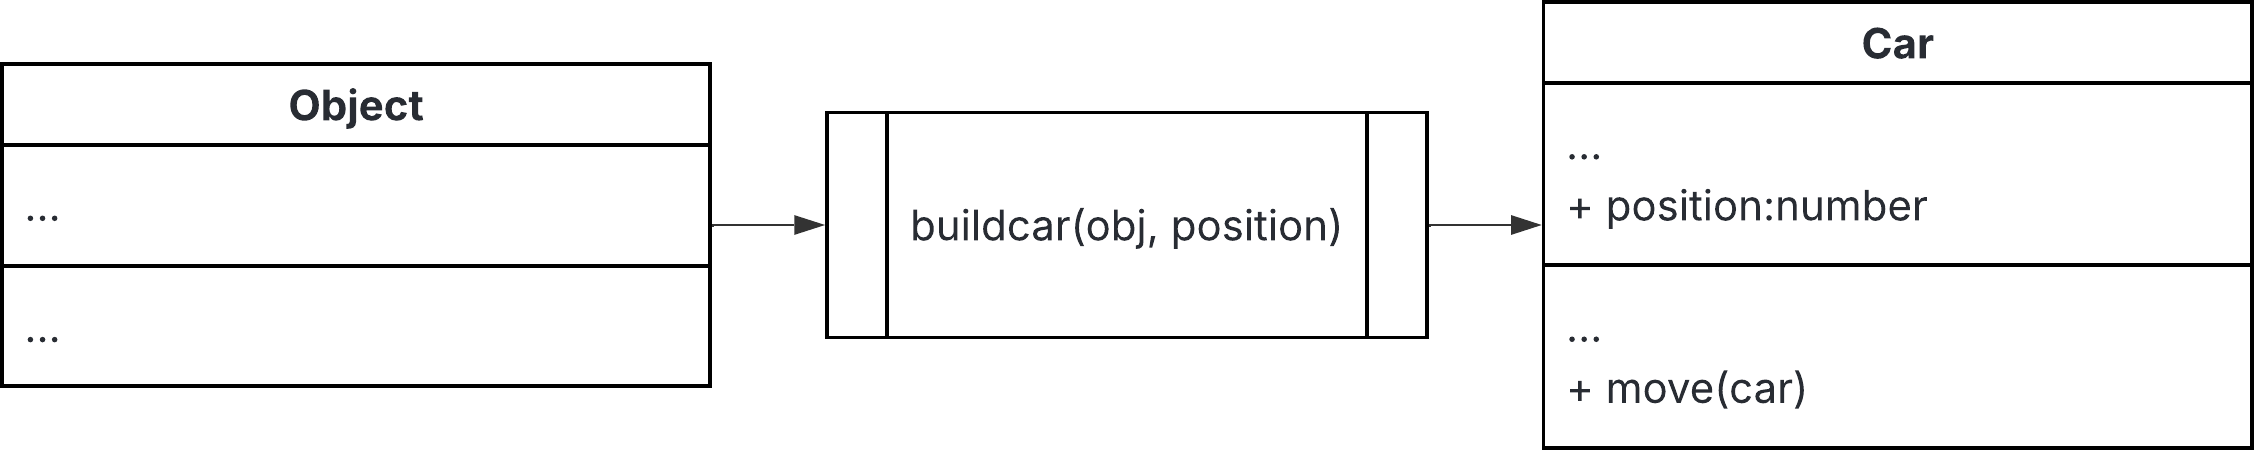
\includegraphics[width=\linewidth]{Images/Decorator 2.png}
    \caption{Example of usage of the decorator function to add an attribute and a method to an object}
    \label{fig:decorator_2}
\end{figure}

While decorators provide runtime flexibility, the systemic shift from augmenting existing instances to creating new ones from a template led to the development of the ``Functional Class'' pattern.

\section{Functional Classes}

The Functional Class pattern was an early attempt to create standardized ``molds'' for similar objects using constructor functions. It aimed to automate the reproduction of objects sharing the same ``type''---possessing identical state structures and methods---while maintaining strong encapsulation through closures.\\

In Functional Classes, unlike in the Decorator Pattern, the \textbf{constructor function} (the function that produce fleets of similar objects) initializes an internal object literal, assigns state and methods to it using passed arguments, and returns that object. This pattern is often chosen to avoid the complexities of the \texttt{this} keyword and the associated risk of \textbf{context loss} (where \texttt{this} inadvertently points to the global object).\\

\textbf{Performance Implications of Method Duplication} From an architectural perspective, the ``So What?'' of this pattern is its inherent memory inefficiency. Because every instance created via a functional class carries a unique copy of its methods, memory consumption grows linearly with the number of instances. This creates high \textbf{GC Pressure}, as the JavaScript engine must periodically spike CPU usage to clean up thousands of identical function objects that could have been shared.

\begin{itemize}
    \item
        \textbf{Pros:}   
        \begin{itemize}
            \item Strong encapsulation via closures (true private state);
            \item Avoids \texttt{this} keyword complexity;
            \item Intuitive syntax.
        \end{itemize}
    
    \item
        \textbf{Cons:}   
        \begin{itemize}
            \item Highly memory inefficient;
            \item Fails the \texttt{instanceof} test because \texttt{Object.getPrototypeOf()} returns a generic \texttt{Object.prototype};
            \item Stripping the object of its architectural identity.
        \end{itemize}
    
    \item
        \textbf{Use Cases:}
        \begin{itemize}
            \item Scenarios requiring absolute state privacy;
            \item Small-scale utilities where performance is secondary to security.
        \end{itemize}
\end{itemize}

\subsection{Example of functional class usage}

Let us make the car object example using this other pattern.

\begin{lstlisting}
    var Car = function(position){
        var obj = {position: position};
        obj.move = function(){
            obj.position++;
        }
        return obj;
    };
    
    var carA = Car(1);
    carA.move();
\end{lstlisting}

Using this pattern, the function does not accept a generic object in input which could have attributes and methods, instead, it creates the object and the assigns it its own function. The schematization of this example is depicted in figure \ref{fig:functional_class}.\\

\begin{figure}
    \centering
    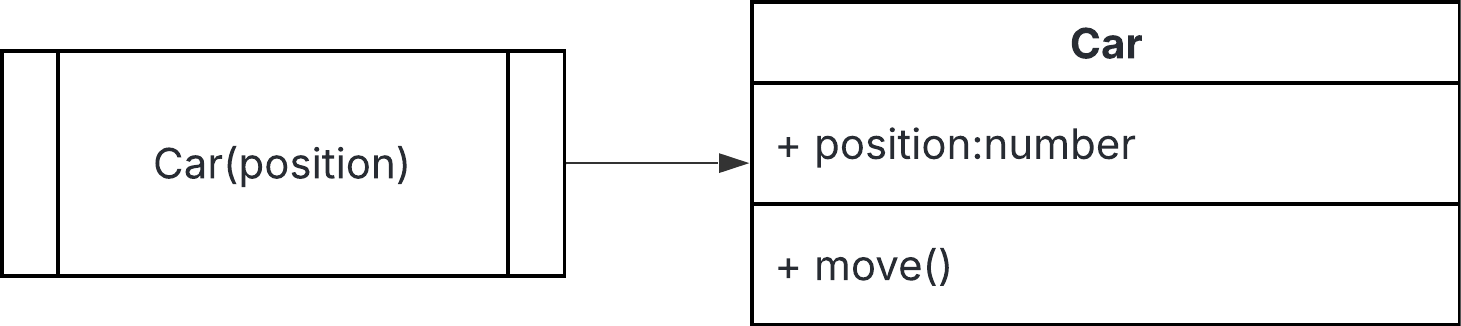
\includegraphics[width=\linewidth]{Images/Functional classes.png}
    \caption{Example of functional class usage}
    \label{fig:functional_class}
\end{figure}

\section{Functional shared pattern}

The functional shared pattern is a variant of the functional class pattern in which object functions are defined externally to the object and the constructor function assigns methods to the objects as references. Defining functions externally is more memory efficient but introduces the complexity related to contexts and the \texttt{this} keyword.\\

Let us understand this pattern better by exposing an example.

\subsection{Example of functional shared pattern usage}

Let us make the car object example as we did using the functional class pattern but defining the \texttt{move} function externally:

\begin{lstlisting}
    var Car = function(position){
        var obj = {position: position};
        obj.move = move;
        return obj;
    };
    
    var move = function(){
        // The move function cannot access obj anymore
        obj.position++;
    };
\end{lstlisting}

This implementation will not work because the \texttt{move} function no longer has closure scope access to the \texttt{obj} variable. We can use this pattern if we implement the \texttt{move} function using the \texttt{this} keyword to refer to the car object.

\begin{lstlisting}
    var Car = function(position){
        var obj = {position: position};
        obj.move = move;
        return obj;
    };
    
    var move = function(){
        this.position++:
    };
    
    var carA = Car(1);
    carA.move();
\end{lstlisting}

This implementation will work because the \texttt{move} function refers to the car object through the \texttt{this} keyword. Notice that the reference to the \texttt{move} function inside the car object is defined as: \texttt{obj.move = move;}. To the left of the \texttt{move} function there is \texttt{obj} which means that the \texttt{this} keyword inside the externally defined \texttt{move} function will refer to \texttt{obj}. The schematization of this example is depicted in figure \ref{fig:functional_shared_pattern}.\\

\begin{figure}
    \centering
    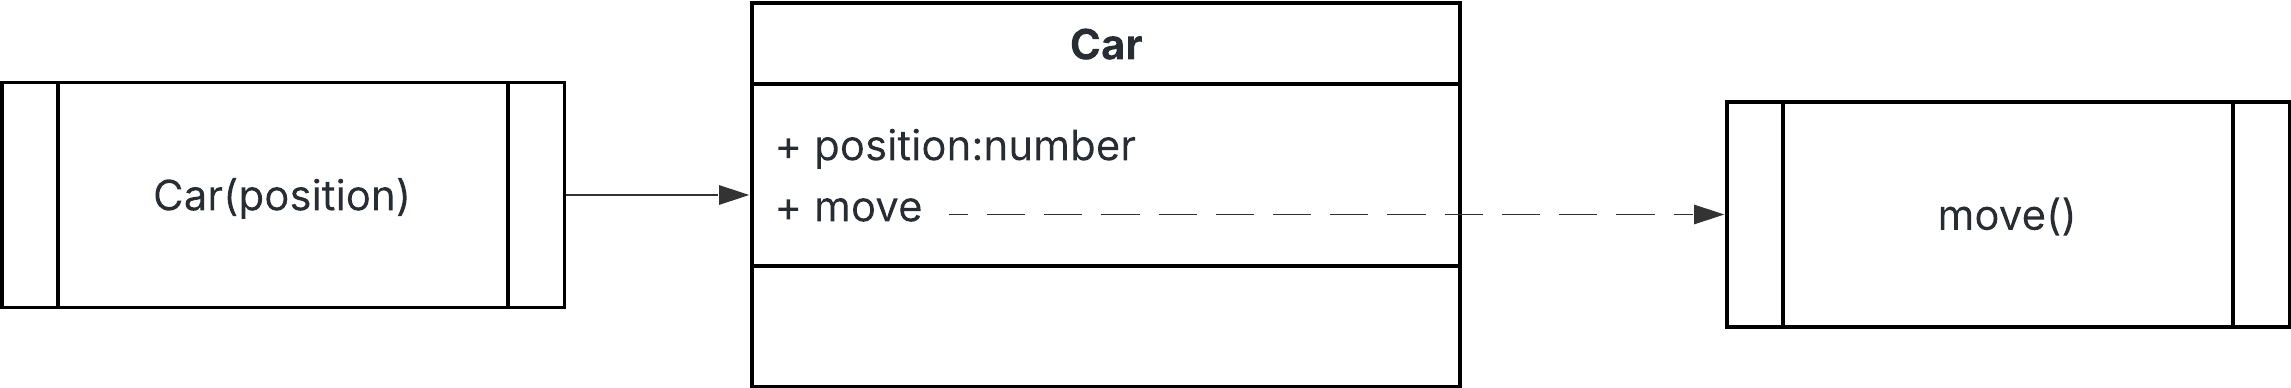
\includegraphics[width=\linewidth]{Images/Functional shared pattern.png}
    \caption{Example of functional shared pattern usage}
    \label{fig:functional_shared_pattern}
\end{figure}

Roughly speaking: the functional shared pattern is a variant of the functional classes pattern in which we define methods externally to the objects to trade off memory efficiency for context management complexity.\\

At this point one might say: what if we want a trade-off between the functional classes pattern and the functional shared pattern? What if, given a class of objects, we only need true encapsulation for some of them while we can afford external definition and memory efficiency for the others? This reasoning is the foundation of the following pattern.

\section{Functional Shared Pattern with Closure (Hybrid Pattern)}

The functional shared patter with closure is a hybrid between the latter two patterns. Given an object we establish which ones must be encapsulated for privacy and define externally all the others for memory efficiency. Let us make an example of hybrid pattern usage.

\subsection{Example of hybrid pattern usage}

Let us say that we want to make a car and a horse object. They both move but only the car can honk and only the horse can neigh. For this reason, we can define the \texttt{move} methods externally and the other two internally.

\begin{lstlisting}
    var Car = function(position){
      var obj = {position: position};
      obj.move = move;
      
      obj.honk = function(){
        console.log("I'm honking the horn!");
      }
      
      return obj;
    }
    
    var Horse = function(position){
      var obj = {position: position};
      obj.move = move;
      
      obj.neigh = function(){
        console.log("Neigh!");
      }
      
      return obj;
    }
    
    var move = function(){
      this.position++;
    };
        
    var carA = Car(1);
    var horse = Horse(1);
    
    carA.move();
    horse.move();
    
    carA.honk();
    horse.neigh();
\end{lstlisting}

In this example in particular we decided to implement methods internally or externally according to a pertinence criterion but in a real life scenario this decision can also depend on privacy and security.\\

The schematization of the example is depicted in figure \ref{fig:hybrid_pattern}.

\begin{figure}
    \centering
    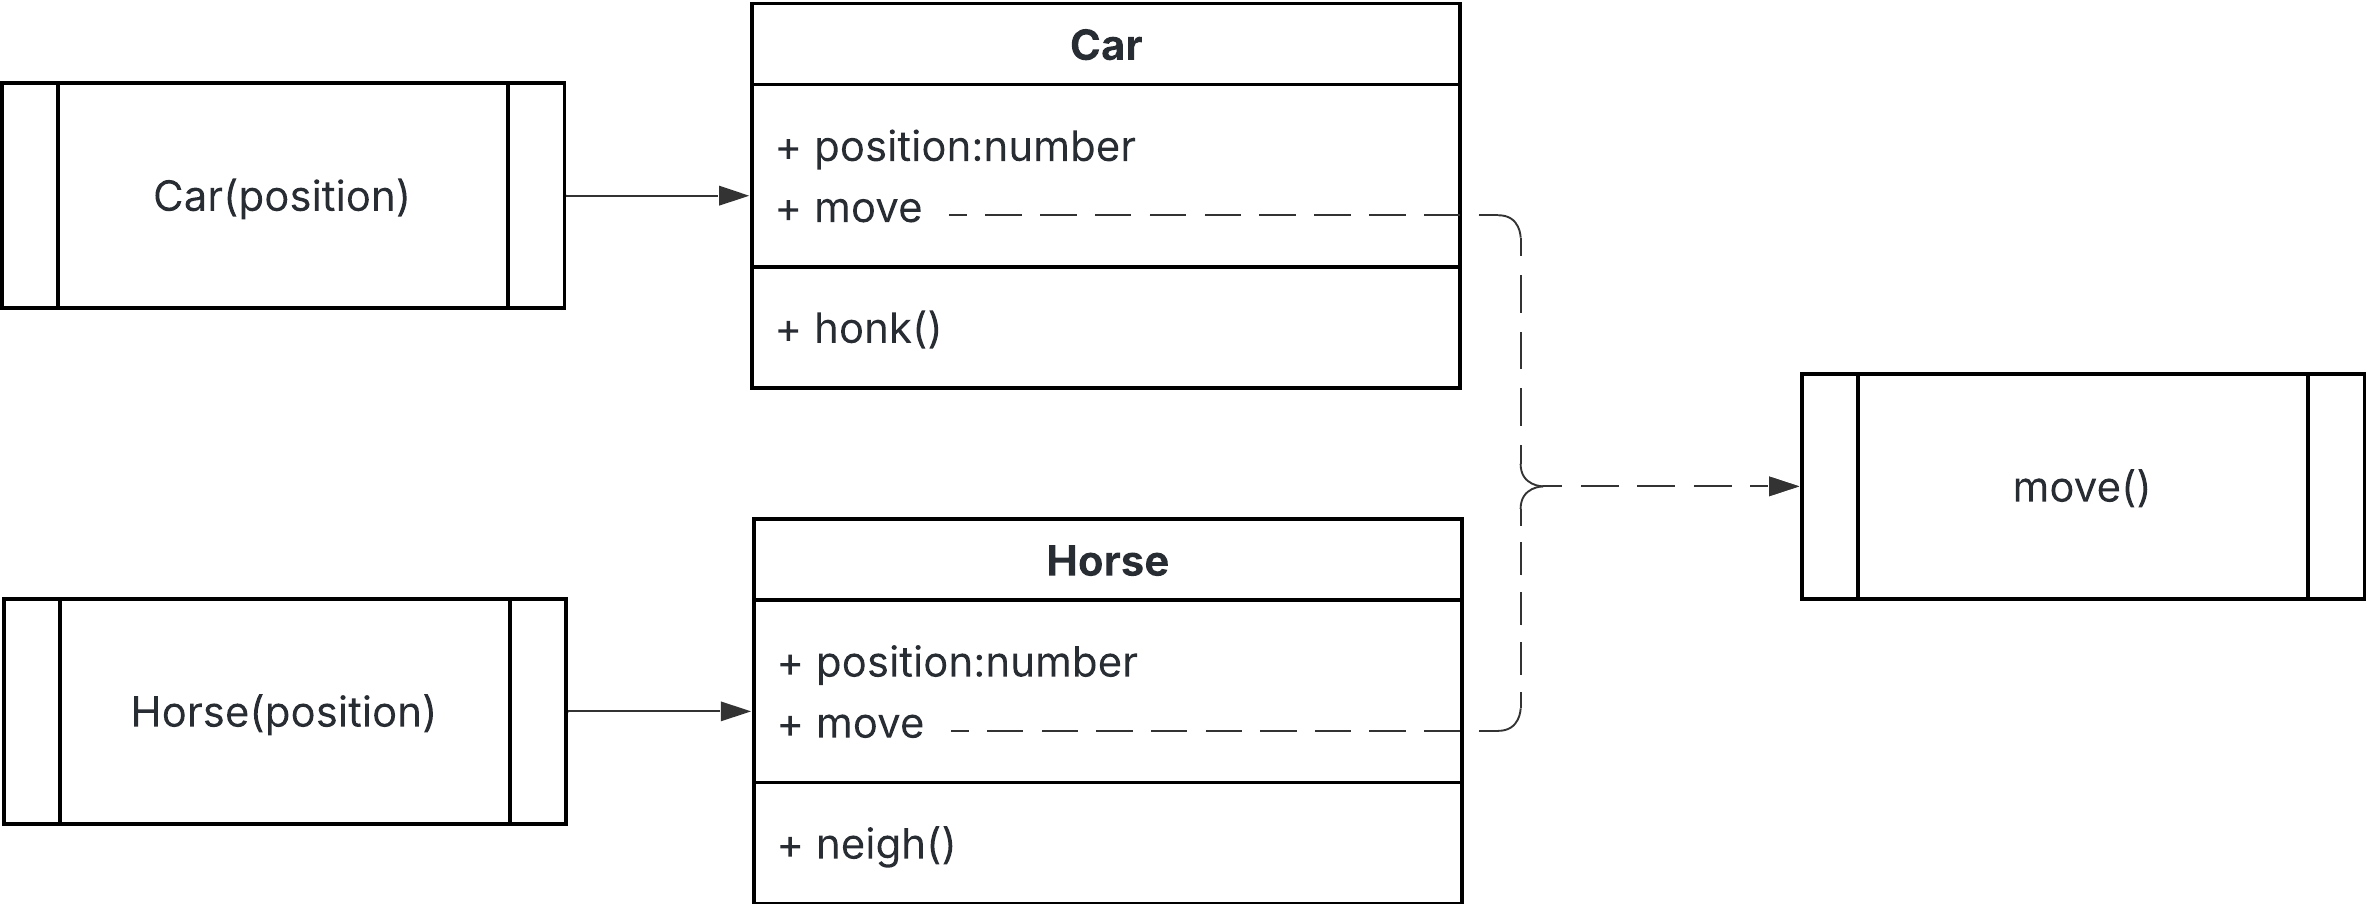
\includegraphics[width=\linewidth]{Images/Hybrid pattern.png}
    \caption{Example of hybrid pattern usage}
    \label{fig:hybrid_pattern}
\end{figure}

\section{Prototypal Classes}

Prototypal classes represent a fundamental shift from ``copying'' to ``delegation.'' In this model, objects are linked to a central repository of methods rather than carrying their own. The implementation uses \texttt{Object.create(prototypeObject)} to link the new instance's internal \texttt{[[Prototype]]} (known in industry jargon as \textbf{dunder proto} or \texttt{\_\_proto\_\_}) to a ``mold'' object.\\

\textbf{The Architectural ``Lookup Chain''} When a method is called on an instance, the engine follows a specific lookup chain: \texttt{Instance => Mold Object (\_\_proto\_\_) => Object.prototype => null}. For example, \texttt{carA => Car.methods => Object => null}. This delegation is vastly superior for memory management, as a single copy of a method can serve thousands of instances.

\begin{itemize}
    \item
        \textbf{Pros:}
        \begin{itemize}
            \item Extreme memory efficiency;
            \item Allows ``live updates'' where modifying the prototype affects all instances immediately.
        \end{itemize}
        
    \item
        \textbf{Cons:}
        \begin{itemize}
            \item More complex syntax;
            \item Requires manual state initialization (often through a secondary \texttt{init} method).
        \end{itemize}
    
    \item
        \textbf{Use Cases:}
        \begin{itemize}
            \item Performance-critical systems;
            \item Applications managing massive entity counts.
        \end{itemize}
\end{itemize}

\subsection{Example of prototypal class usage}

\begin{lstlisting}
    var Car = function(position){
      var obj = Object.create(Car.methods);
      obj.position = position;
      return obj;
    };
    
    Car.methods = {
      move: function(){
        this.position++;
      }
    };
    
    var carA = Car(1);
    carA.move();

    // Prototype chain test
    console.log(carA.__proto__); // Car.methods
    console.log(carA.__proto__.__proto__); // Object
    console.log(carA.__proto__.__proto__.__proto__); // null
\end{lstlisting}

In this example we have a constructor function which creates \texttt{obj} by assigning the object \texttt{Car.methods} as its prototype. The \texttt{move} function, which is common to all the objects, is assigned to the \texttt{Car.methods} object to leverage the prototype chain. This strategy avoids copying the function saving space and time.\\

At the end of the code, we can see the prototype chain in action. The schematization of this pattern is depicted in figure \ref{fig:prototypal_classes}.\\

\begin{figure}
    \centering
    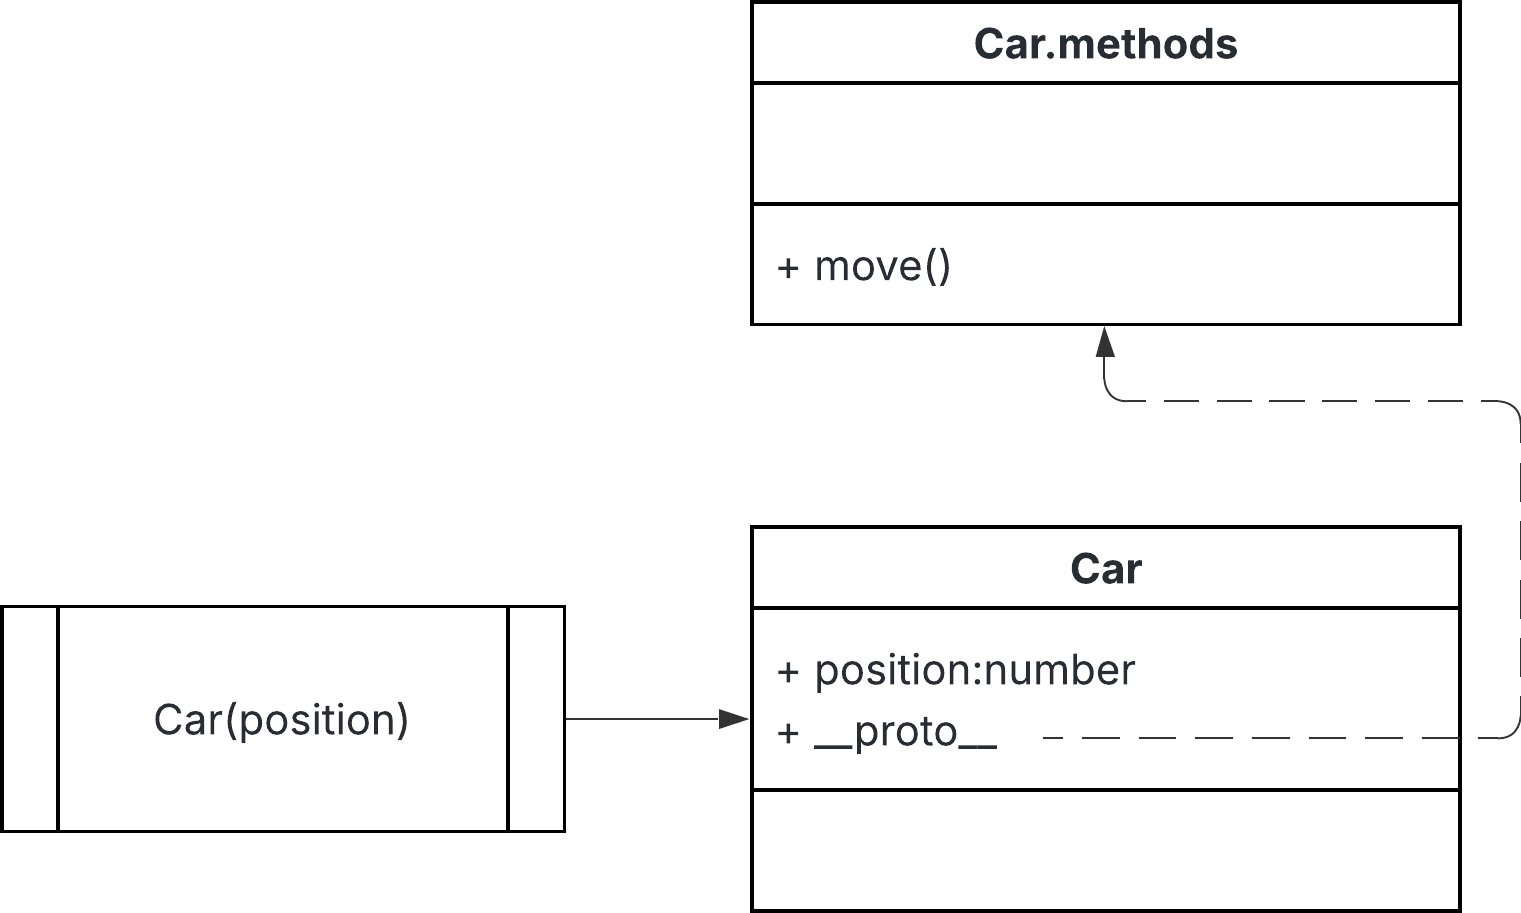
\includegraphics[width=0.5\linewidth]{Images/Prototypal classes.png}
    \caption{Example of prototypal classes usage}
    \label{fig:prototypal_classes}
\end{figure}

\subsection{Example of prototypal class usage with official conventions}

Since this pattern is so common, the language designer decided to add official conventions to support it. Instead of creating a new object (\texttt{Car.methods} in the previous example), we can leverage the default existing one which is called \texttt{Car.prototype}. The prototype object comes by default when we create an object and has a \texttt{constructor} property which stores a pointer to the function it comes attached to which, in our example, is \texttt{Car}.

\begin{lstlisting}
    var Car = function(position){
      var obj = Object.create(Car.prototype);
      obj.position = position;
      return obj;
    };
    
    Car.prototype.move = function(){
      this.position++;
    };
    
    var carA = Car(1);
    carA.move();
    
    // Prototype chain test
    console.log(carA.__proto__); // Car.prototype
    console.log(carA.__proto__.__proto__); // Object
    console.log(carA.__proto__.__proto__.__proto__); // null
    
    // Constructor test
    console.log(Car.prototype.constructor); // Car
\end{lstlisting}

This code is basically the same as the one of the previous example but we use the default object instead of creating a new one. At the end of the snippet there is also a constructor test to check if the constructor property of the prototype object points back to the \texttt{Car} object. The schematization of this pattern is depicted in figure \ref{fig:prototypal_classes_official_convention}.

\begin{figure}
    \centering
    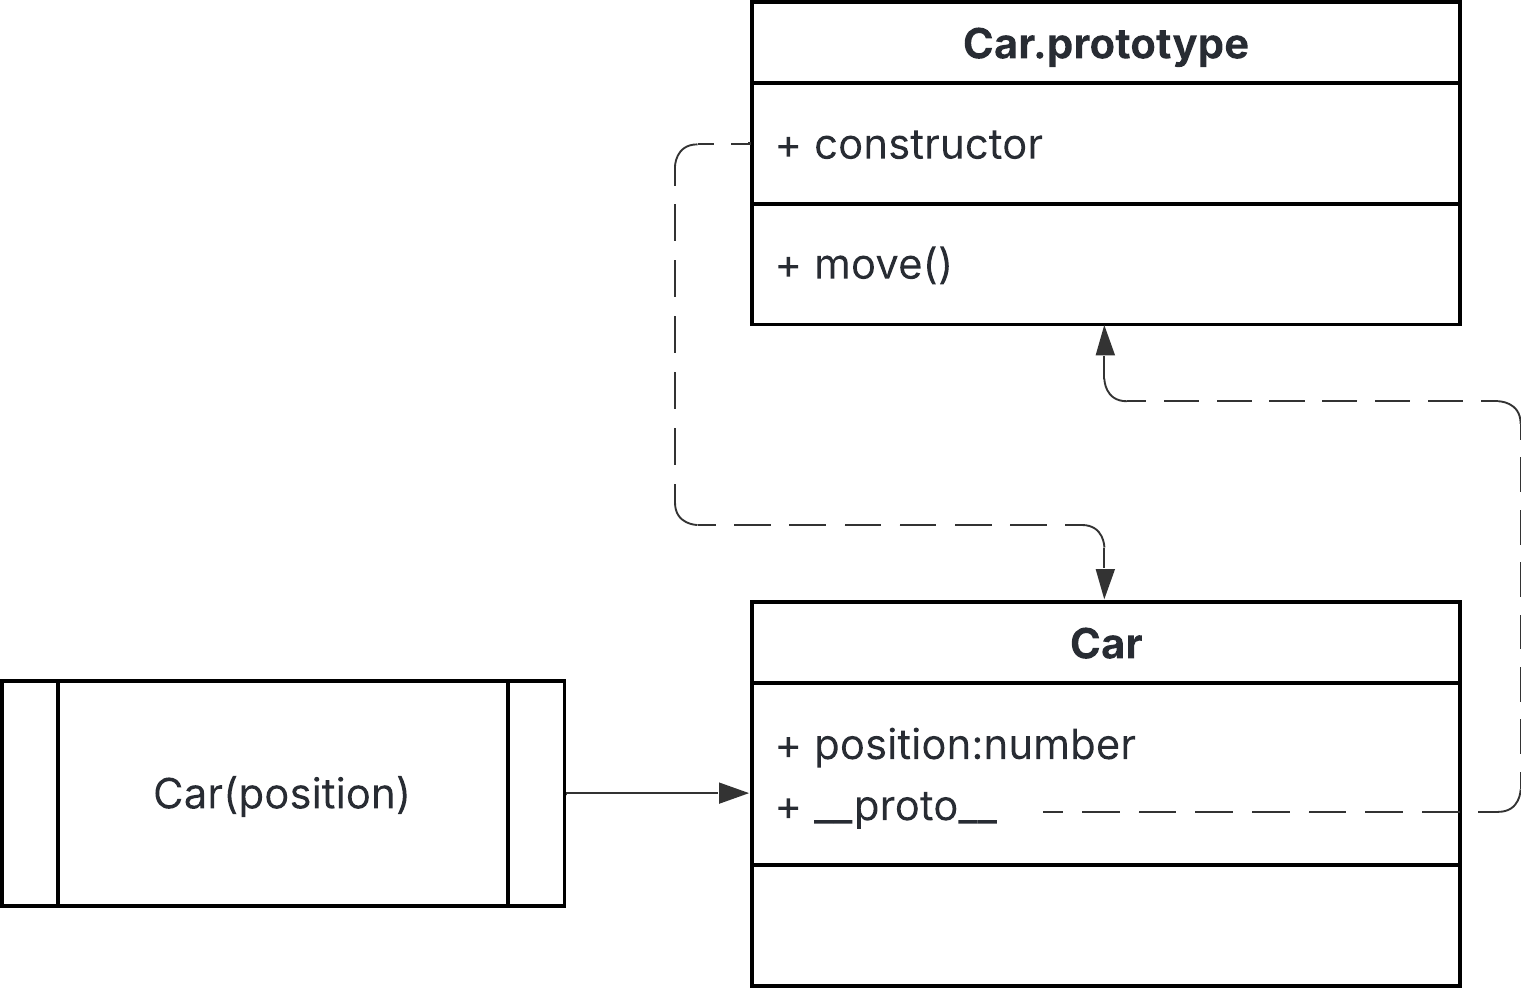
\includegraphics[width=0.5\linewidth]{Images/Prototypal classes official.png}
    \caption{Example of prototypal classes usage with official convention}
    \label{fig:prototypal_classes_official_convention}
\end{figure}

\section{The Pseudoclassical Pattern}

The Pseudoclassical pattern is the standard bridge between traditional class-based expectations and JavaScript's prototypal reality. It uses constructor functions and the \texttt{new} keyword to provide an interface familiar to those from Java or C++ backgrounds while leveraging the efficiency of prototypes.\\

The \texttt{new} keyword in front of a function invocation triggers the \textbf{Constructor Mode}. In this mode the JavaScript engine executes four precise operations:

\begin{enumerate}
    \item \textbf{Creation:} A new empty object \texttt{\{\}} is created.
    \item \textbf{Linking:} The object's \texttt{[[Prototype]]} is linked to the constructor function's \texttt{.prototype} property.
    \item \textbf{Binding:} The execution context (\texttt{this}) is bound to the new object.
    \item \textbf{Return:} The object is implicitly returned.
\end{enumerate}

These operations are abstracted for syntactic convenience considering that they are recurrent and standardized in the prototypal class pattern.\\

\textbf{JIT Optimization and Predictability} Modern JIT engines like V8 are specifically optimized for this pattern. Because the structure is predictable, the engine can optimize method lookups and property access more effectively than with the ``strange'' or dynamic structures found in functional patterns. Predictability is the primary driver of performance in high-scale JavaScript.

\begin{itemize}
    \item
        \textbf{Pros:}    
        \begin{itemize}
            \item Standardized;
            \item Memory-efficient;
            \item Compatible with \texttt{instanceof};
            \item Highly optimized by V8.
        \end{itemize}
    
    \item
        \textbf{Cons:}
        \begin{itemize}
            \item Fragile if \texttt{new} is omitted (context loss);
            \item Syntax for manual prototype attachment is verbose.
        \end{itemize}
    
    \item
        \textbf{Use Cases:} General application logic and framework development.
\end{itemize}

\subsection{Example of pseudoclassical pattern usage}

\begin{lstlisting}
    var Car = function(position){
      this.position = position;
    };
    
    Car.prototype.move = function(){
      this.position++;
    };
    
    var carA = new Car(1);
    carA.move();
    
    console.log(carA instanceof Car); // true
\end{lstlisting}

This is the implementation of our car example using the pseudoclassical pattern. Notice that in the constructor function there aren't the empty object creation and the return statement returning the object because these operations are abstracted by the JavaScript engine.\\

At the end of the snippet there is a test which verifies that the newly created object is considered an instance of the \texttt{Car} class.

\section{Superclasses and Subclasses}

Inheritance establishes ``is-a'' relationships, allowing a subclass to inherit the logic of a parent superclass. This requires a two-pronged strategy:

\begin{enumerate}
    \item \textbf{Constructor Stealing:} The subclass invokes the superclass constructor to initialize base state on the subclass instance.
    \item \textbf{Behavior Delegation:} The subclass links its prototype to the superclass prototype to inherit methods.
\end{enumerate}

\subsection{Example of superclasses and subclasses usage}

Let us say that we have two constructor functions for the \texttt{Van} class and for the \texttt{Cop} class defined as follows:

\begin{lstlisting}
    var Van = function(position){
        var obj = {position: position};
        obj.move = function(){ obj.position++; };
        obj.grab = function(){/*...*/};
        return obj;
    };
    
    var Cop = function(position){
        var obj = {position: position};
        obj.move = function(){ obj.position++; };
        obj.call = function(){/*...*/};
        return obj;
    };
\end{lstlisting}

These two constructor functions have duplicate code. This not only makes the constructor functions more complicated and heavier than they could be but also creates maintenance issues because if we want to update the common part of both functions we would have to make the same changes to both the functions. This process is error prone and can be avoided by creating a superclass containing the common code of both functions. After we create a superclass, we can use the object it creates as a starting point for the subclasses which will have to implement only their unique codes.\\

In this example in the specific we can define a \texttt{Car} class to implement the common code and simplify the other classes as follows.

\begin{lstlisting}
    var Car = function(position){
        var obj = {position: position};
        obj.move = function(){
            obj.position++;
        };
        return obj;
    };

    var Van = function(position){
        var obj = Car(position);
        obj.grab = function(){/*...*/};
        return obj;
    };

    var Cop = function(position){
        var obj = Car(position);
        obj.call = function(){/*...*/};
        return obj;
    };
\end{lstlisting}

The schematization of this pattern is depicted in figure \ref{fig:superclass_subclass}.

\begin{figure}
    \centering
    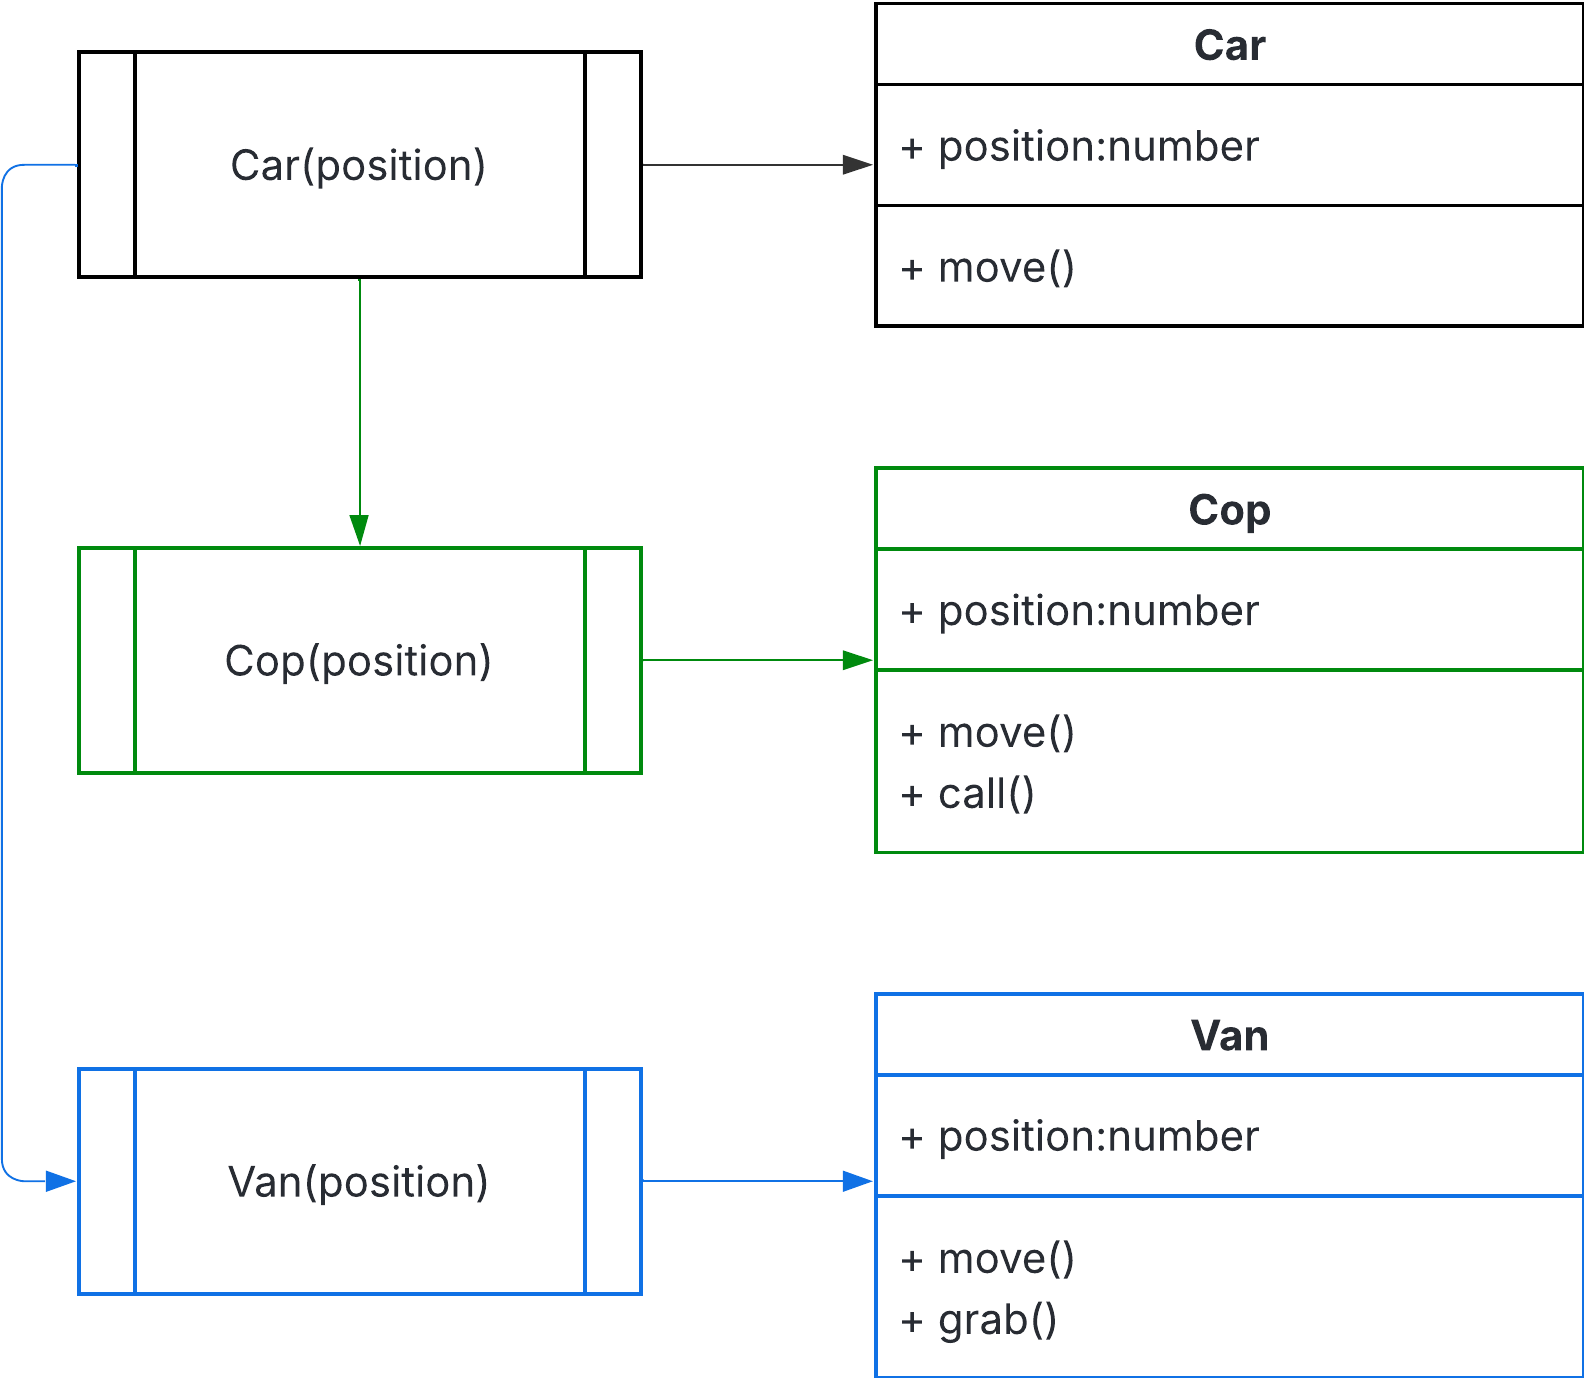
\includegraphics[width=0.5\linewidth]{Images/Superclasses and subclasses.png}
    \caption{Example of superclasses and subclasses usage}
    \label{fig:superclass_subclass}
\end{figure}

\section{Pseudoclassical Subclasses}

Implementing subclasses pseudoclassically is technically demanding, as missing a single step in the boilerplate can break the inheritance chain or lead to identity errors.\\

The implementation requires three critical steps:

\begin{enumerate}
    \item \textbf{Invoke Super:} Use \texttt{Superclass.call(this [, args])} inside the subclass constructor.
    \item \textbf{Link Prototypes:} Set \texttt{Subclass.prototype = Object.create(Superclass.prototype)}.
    \item \textbf{Reset Constructor:} Manually set \texttt{Subclass.prototype.constructor = Subclass}. This is the most common point of failure; without this reset, the \texttt{constructor} property will incorrectly point to the superclass.
\end{enumerate}

\begin{itemize}
    \item
        \textbf{Pros:}
        \begin{itemize}
            \item Full inheritance support;
            \item High memory efficiency;
            \item Clear type checking.
        \end{itemize}
    
    \item
        \textbf{Cons:}
        \begin{itemize}
            \item Verbose boilerplate;
            \item Error-prone manual linking.
        \end{itemize}
    
    \item \textbf{Use Cases:} Hierarchical domain models (e.g., \texttt{Vehicle} $\rightarrow$ \texttt{Car}).
\end{itemize}

\subsection{Example of pseudoclassical subclasses usage}

\subsubsection{Pseudoclassical pattern problems analysis}

Let us start from the analysis of the problems of the pseudoclassical pattern.

\begin{lstlisting}
    var Car = function(position){
      this.position = position;
    };
    
    Car.prototype.move = function(){
      this.position++;
    };
    
    var Van = function(position){
      // Without the keyword 'new' obj is undefined
      var obj = new Car(position);
      
      obj.grab = function(){
        console.log("I'm grabbing!");
      }

      // If we don't return the object, vanA is undefined.
      return obj;
    };
    
    var vanA = new Van(3);
    vanA.move();
    vanA.grab();
    
    console.log(vanA.__proto__ === Van.prototype); // false
    console.log(vanA.__proto__ === Car.prototype); // true
    console.log(vanA instanceof Van); // false
    console.log(vanA instanceof Car); // true
\end{lstlisting}

This approach requires us to pay particular attention to the boilerplate of the code rather than the business logic. In fact, skipping the \texttt{new} or \texttt{return} keyword causes the code not to work as described in the comments of the code. Furthermore, the prototype chain is deceitful because one might think that the prototype of \texttt{vanA} is \texttt{Van.prototype} and \texttt{vanA} is an instance of \texttt{Van}. Instead, the \texttt{Van} object is decorated \texttt{Car} object.\\

The schematization of this implementation is depicted in figure \ref{fig:pseudoclassical_subclasses_1}.\\

\begin{figure}
    \centering
    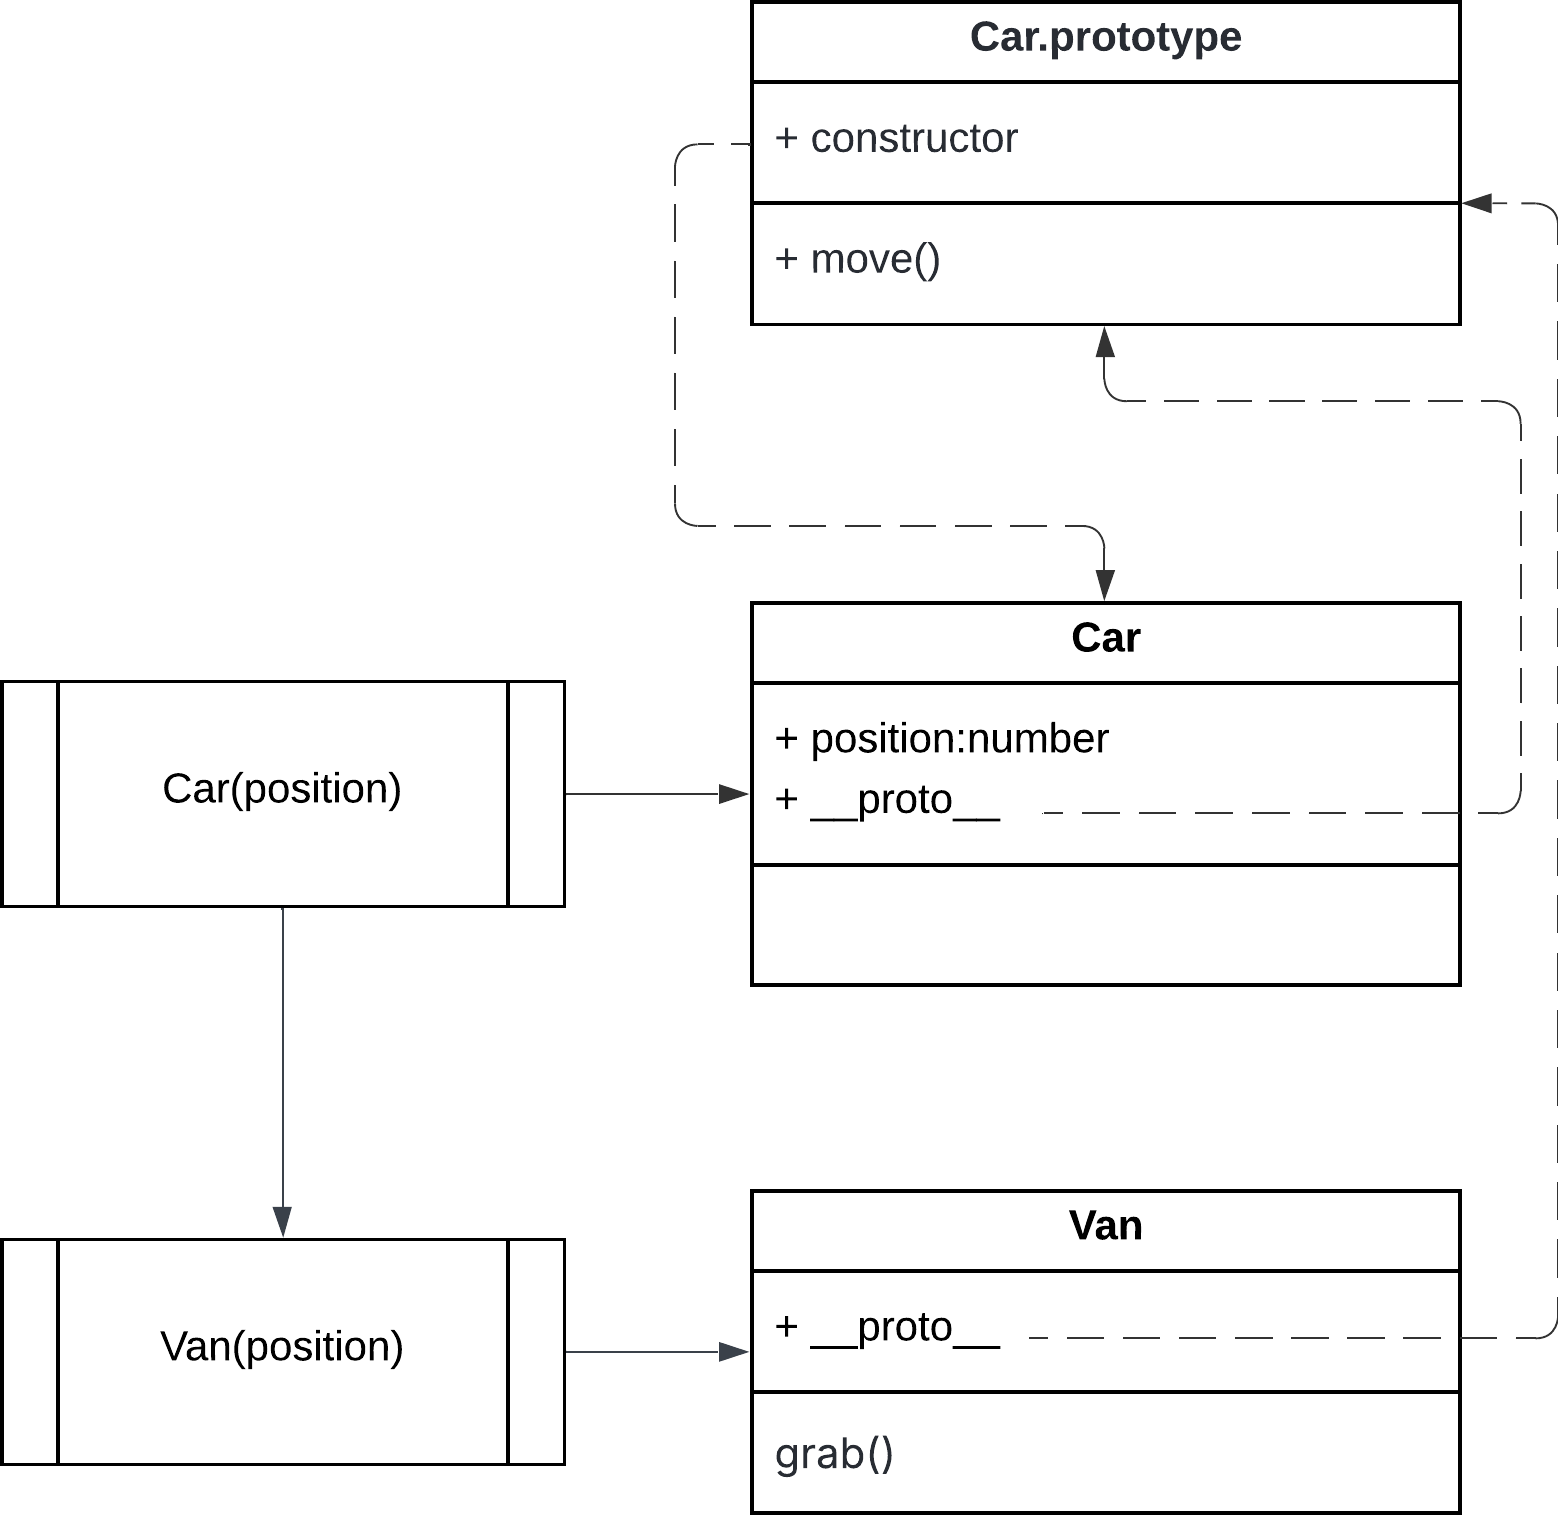
\includegraphics[width=0.5\linewidth]{Images/Pseudoclassical subclasses 1.png}
    \caption{Example highlighting the problems of the pseudoclassical pattern}
    \label{fig:pseudoclassical_subclasses_1}
\end{figure}

\subsubsection{Setting the execution context using the Superclass.call function}

We can partially address the problems of the pseudoclassical pattern by using \texttt{Superclass.call(this [, args])} to explicitly control the execution context of the superclass constructor. In this case, we invoke \texttt{Car} in the context of the object being created by \texttt{Van} which means that we execute the constructor of \texttt{Car} in the context of the current object \texttt{Van}.

\begin{lstlisting}
    var Car = function(position){
      this.position = position;
    };
    
    Car.prototype.move = function(){
      this.position++;
    };
    
    var Van = function(position){
      Car.call(this, position);
      
      this.grab = function(){
        console.log("I'm grabbing!");
      }
    };
    
    var vanA = new Van(3);
    // vanA.move(); // ERROR
    vanA.grab();
    console.log("Van position: " + vanA.position);
    
    var carA = new Car(1);
    carA.move();
    // carA.grab(); // ERROR
    console.log("Car position: " + carA.position);
    
    console.log(vanA.__proto__ === Van.prototype); // true
    console.log(vanA.__proto__ === Car.prototype); // false
    console.log(vanA.__proto__ === Car); // false
    console.log(vanA instanceof Van); // true
    console.log(vanA instanceof Car); // false
\end{lstlisting}

When executing this code, we encounter two errors. The first one occurs at \texttt{vanA.move();}. Although we invoked the superclass constructor using \texttt{Car.call(this, position)}, this operation only initializes the current object (i.e., the instance created by \texttt{new Van}) by assigning its properties. It does not establish any link between \texttt{Van.prototype} and \texttt{Car.prototype}. As a consequence, the method \texttt{move}, which is defined on \texttt{Car.prototype}, is not accessible from \texttt{vanA}. In other words, \texttt{call} allows us to reuse the constructor logic of the superclass, but it does not implement inheritance. The prototype chain remains unchanged, and therefore \texttt{Van} is not yet a subclass of \texttt{Car}.\\

The second error occurs at \texttt{carA.grab();}. This highlights another important aspect: methods defined inside the \texttt{Van} constructor (such as \texttt{grab}) are assigned directly to instances of \texttt{Van} and are not shared with instances of \texttt{Car}. Even though \texttt{Car.call} is used within \texttt{Van}, it does not introduce any relationship in the opposite direction. Therefore, \texttt{Car} instances cannot access methods defined in \texttt{Van}.\\

Finally, the prototype tests confirm the situation. The object \texttt{vanA} is correctly recognized as an instance of \texttt{Van}, and its internal \texttt{\_\_proto\_\_} points to \texttt{Van.prototype}. However, since there is no delegation from \texttt{Van.prototype} to \texttt{Car.prototype}, \texttt{vanA} is not an instance of \texttt{Car} and cannot access its prototype methods.\\

The schematization of this implementation is depicted in figure \ref{fig:pseudoclassical_subclasses_2}. The figure highlights that the two objects and their relative prototype chains are separated and there isn't an inheritance relationship between \texttt{Van} and \texttt{Car}.

\begin{figure}
    \centering
    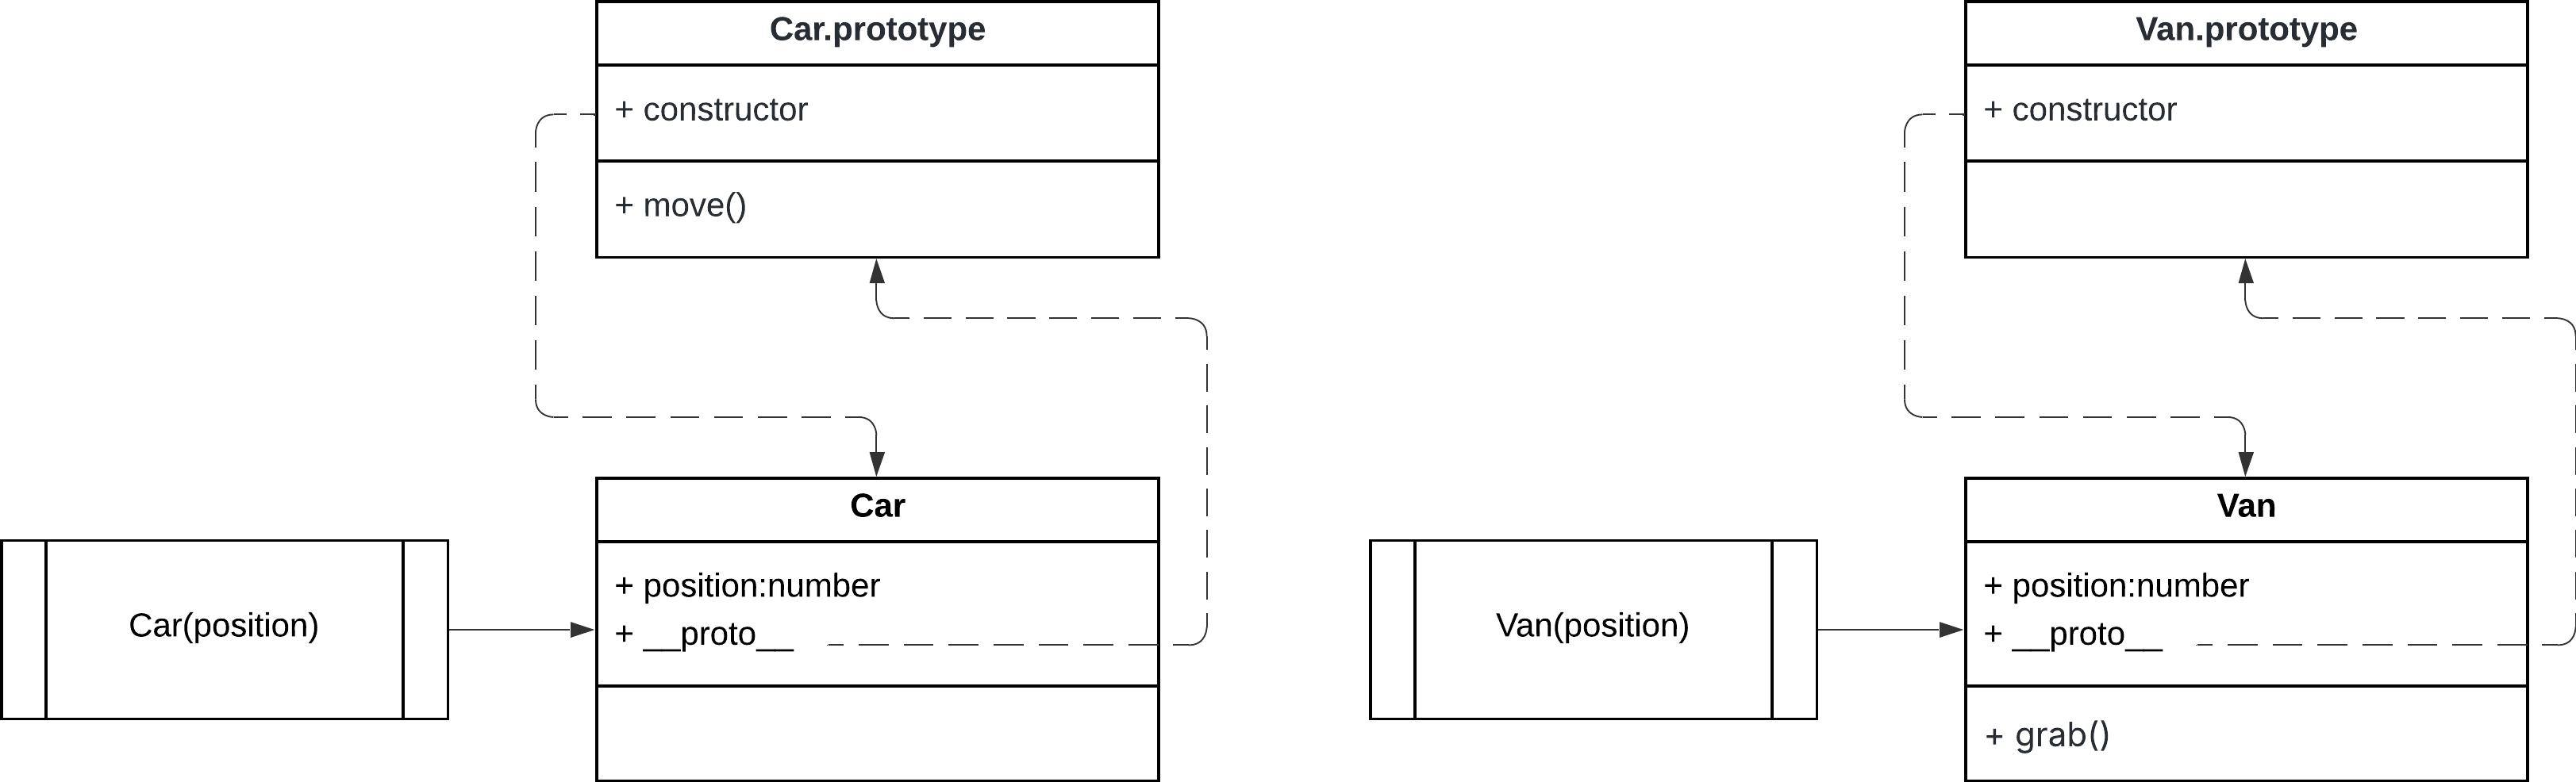
\includegraphics[width=\linewidth]{Images/Pseudoclassical subclasses 2.png}
    \caption{Example of \texttt{Superclass.call} function usage to partially solve the problem}
    \label{fig:pseudoclassical_subclasses_2}
\end{figure}

\subsubsection{Fixing the prototype chain}

We can ultimately solve the problem by fixing the prototype chain manually. We need to first create a prototype object for \texttt{Van} and then set the \texttt{constructor} pointer of the newly created object to the \texttt{Van} class.

\begin{lstlisting}
    var Car = function(position){
      this.position = position;
    };
    
    Car.prototype.move = function(){
      this.position++;
    };
    
    var Van = function(position){
      Car.call(this, position);
      
      this.grab = function(){
        console.log("I'm grabbing!");
      }
    };
    
    /*
      We create a new prototype object for Van that delegates to Car.prototype.
      This does NOT copy Car.prototype, but links the two prototype chains.
    */
    Van.prototype = Object.create(Car.prototype);
    
    console.log(Van.prototype.constructor); // Car
    
    // We set the constructor pointer to the subclass
    Van.prototype.constructor = Van;
    console.log(Van.prototype.constructor); // Van
    
    var vanA = new Van(3);
    vanA.move();
    
    var carA = new Car(1);
    carA.move();
    
    console.log(vanA.__proto__ === Van.prototype); // true
    console.log(vanA.__proto__ === Car.prototype); // false
    console.log(vanA.__proto__ === Car); // false
    console.log(Van.prototype === Car.prototype); // false
    console.log(Van.prototype.__proto__ === Car.prototype); // true
    
    console.log(vanA instanceof Van); // true
    console.log(vanA instanceof Car); // true
\end{lstlisting}

The reason why we use the \texttt{Van.prototype = Object.create(Car.prototype);} is clear: we want to implement prototypal inheritance between \texttt{Van} and \texttt{Car}. But why do we need to set the constructor of the newly created prototype back to the subclass? Doesn't \texttt{Van.prototype} has a \texttt{constructor} variable that points to \texttt{Van} by default?\\

If we leave \texttt{Van.prototype} unchanged, it has a \texttt{constructor} variable that points to \texttt{Van} by default. But when we use the \texttt{create} function we completely replace the default object it used to be and we have an object which only has a pointer to its prototype.

\begin{lstlisting}
    Van.prototype = {
      __proto__: Car.prototype
    }
\end{lstlisting}

This intermediate and unintended state is depicted in figure \ref{fig:pseudoclassical_subclasses_3}.\\

\begin{figure}
    \centering
    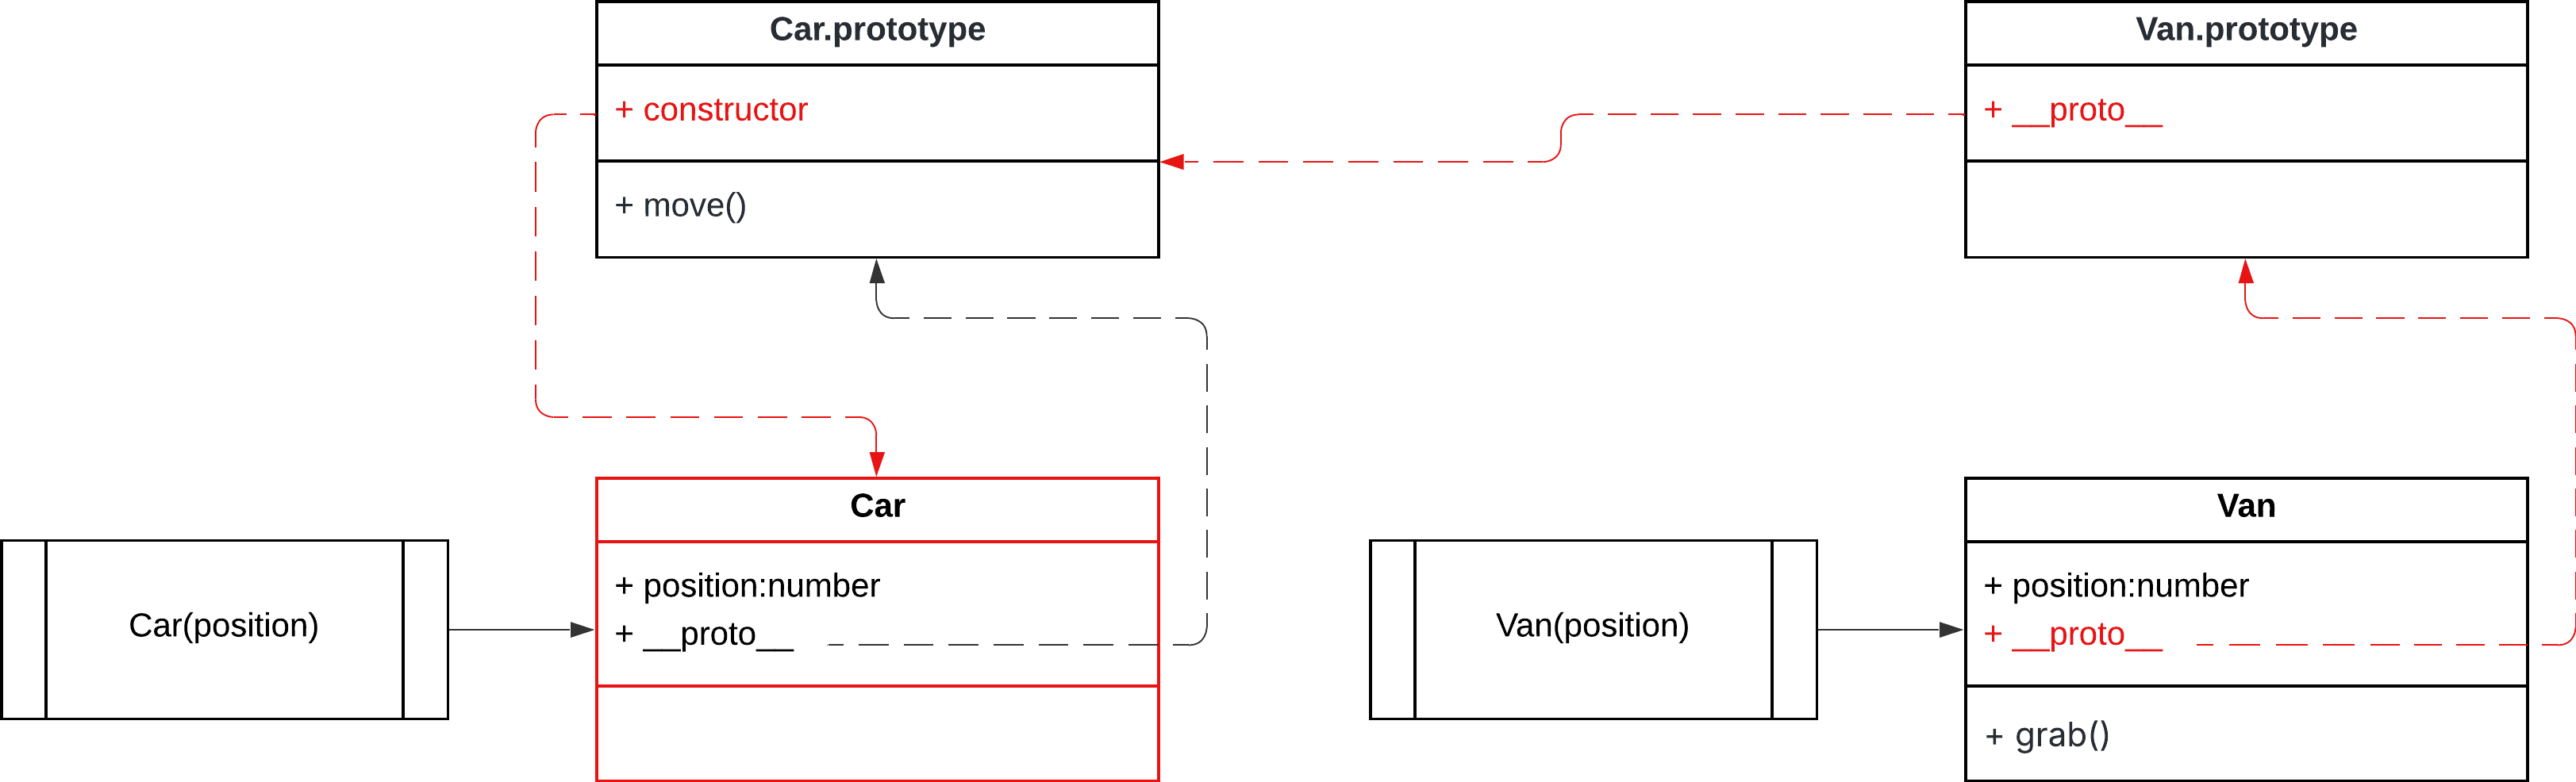
\includegraphics[width=\linewidth]{Images/Pseudoclassical subclasses 3.png}
    \caption{Intermediate problematic state of the pseudoclassical subclasses pattern}
    \label{fig:pseudoclassical_subclasses_3}
\end{figure}

When we call \texttt{Van.prototype.constructor}, the object cannot find the property we are looking for and the request is passed to its prototype i.e. \texttt{Car.prototype}. This object has the \texttt{constructor} property pointing to \texttt{Car} and therefore returns this information. We don't want this to happen so we have to add the \texttt{constructor} property to the newly created \texttt{Van.prototype} object and set it to \texttt{Van}.\\

The final state working as intended is schematized in figure \ref{fig:pseudoclassical_subclasses_4}.

\begin{figure}
    \centering
    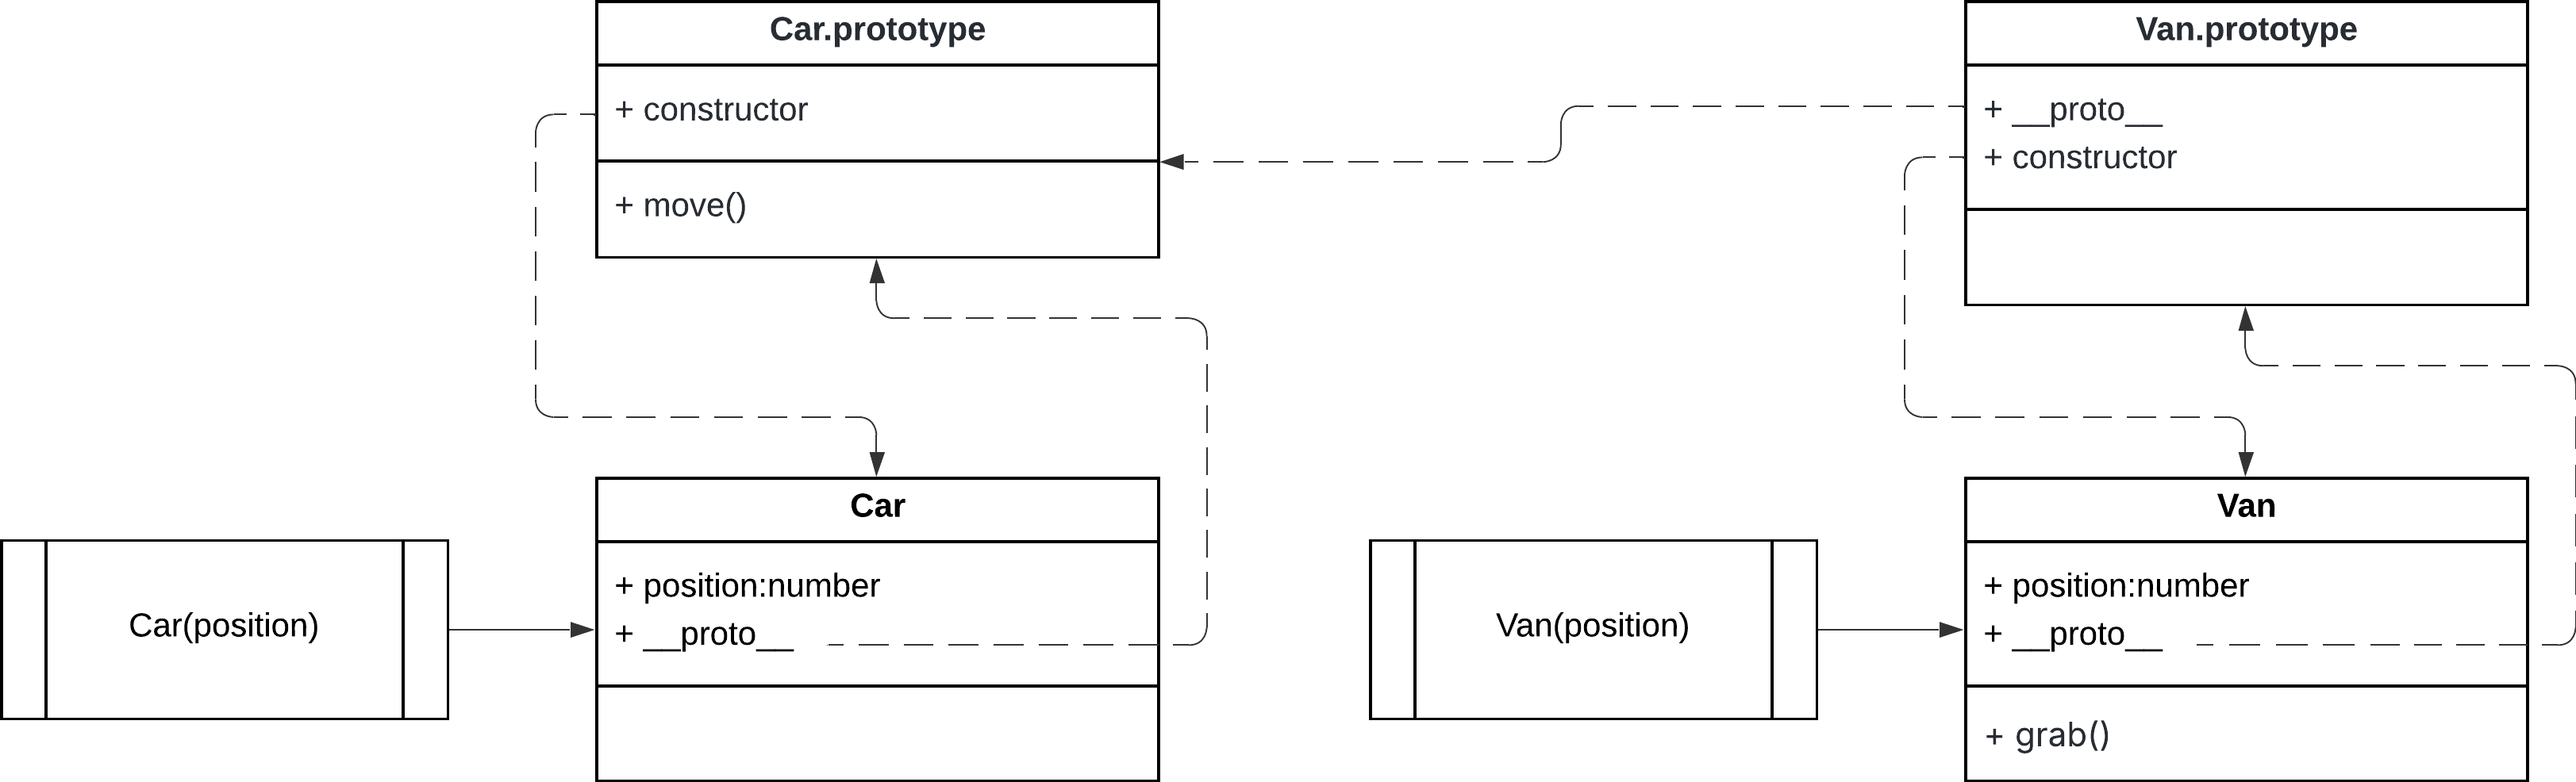
\includegraphics[width=\linewidth]{Images/Pseudoclassical subclasses 4.png}
    \caption{Final state of the pseudoclassical subclasses pattern}
    \label{fig:pseudoclassical_subclasses_4}
\end{figure}

\section{The ES6 Class-based Pattern}

The ES6 Class-based pattern introduces a higher-level abstraction over JavaScript's prototypal inheritance model. It uses the \texttt{class} syntax along with the \texttt{extends} and \texttt{super} keywords to provide a more familiar and structured way to define classes and subclasses.\\

Despite its appearance, this pattern does not introduce true classes. Instead, it is syntactic sugar over the pseudoclassical subclasses pattern, internally relying on prototypes and delegation.\\

The \texttt{extends} keyword establishes inheritance between two classes by linking the prototype of the subclass to the prototype of the superclass. The \texttt{super} keyword is used to invoke the constructor of the superclass and to access its methods.

\begin{enumerate}
    \item \textbf{Class Declaration:} Defines a constructor and its associated methods in a compact syntax.
    \item \textbf{Inheritance:} The \texttt{extends} keyword automatically sets up the prototype chain between subclass and superclass.
    \item \textbf{Super Invocation:} The \texttt{super(...args)} call ensures proper initialization of inherited properties.
    \item \textbf{Method Sharing:} Methods are automatically placed on the class prototype, ensuring memory efficiency.
\end{enumerate}

This abstraction eliminates the need for manual prototype manipulation (e.g., \texttt{Object.create}) and constructor resetting, reducing the likelihood of errors and improving code readability.\\

\textbf{JIT Optimization and Predictability} Modern JavaScript engines optimize class-based code similarly to the pseudoclassical pattern. The structured and declarative nature of classes improves predictability, enabling efficient method dispatch and property access.

\begin{itemize}
    \item
        \textbf{Pros:}
        \begin{itemize}
            \item Cleaner and more expressive syntax;
            \item Built-in support for inheritance via \texttt{extends};
            \item Eliminates manual prototype linking;
            \item Reduces common errors (e.g., missing \texttt{new}, incorrect constructor references);
            \item Fully compatible with \texttt{instanceof}.
        \end{itemize}
    
    \item
        \textbf{Cons:}
        \begin{itemize}
            \item Still based on prototypes (can obscure underlying behavior);
            \item Less flexible than lower-level patterns;
            \item Requires understanding of \texttt{this} and \texttt{super};
            \item May give a misleading impression of classical inheritance.
        \end{itemize}
    
    \item
        \textbf{Use Cases:}
        \begin{itemize}
            \item Large-scale applications;
            \item Hierarchical models;
            \item Codebases requiring readability and maintainability.
        \end{itemize}
\end{itemize}

\subsection{Example of Class-Based Pattern usage}

Let us rewrite the previous example using the Class-Based Pattern syntax.

\begin{lstlisting}
    class Car {
      constructor(position){
        this.position = position;
      }
    
      move(){
        this.position++;
      }
    }
    
    class Van extends Car {
      constructor(position){
        super(position); // equivalent to Car.call(this, position)
    
        this.grab = function(){
          console.log("I'm grabbing!");
        }
      }
    }
    
    // In ES6 classes, the constructor is automatically set correctly
    console.log(Van.prototype.constructor); // Van
    
    var vanA = new Van(3);
    vanA.move();
    
    var carA = new Car(1);
    carA.move();
    
    // Prototype chain check
    console.log(vanA.__proto__ === Van.prototype); // true
    console.log(vanA.__proto__ === Car.prototype); // false
    console.log(vanA.__proto__ === Car); // false
    console.log(Van.prototype === Car.prototype); // false
    console.log(Van.prototype.__proto__ === Car.prototype); // true
    
    // instanceof check
    console.log(vanA instanceof Van); // true
    console.log(vanA instanceof Car); // true
\end{lstlisting}

At the end of the code we have the prototype chain check confirming that this notation is syntactic sugar over the pseudoclassical subclasses pattern. There is also the \texttt{instanceof} check confirming that the JavaScript engine recognizes that the \texttt{vanA} object belongs to both classes.

\section{Synthesis and Pattern Comparison Summary}

\subsection{Architectural Comparison Matrix}

\begin{table}[h]
    \centering
    \tiny
    \begin{tabularx}{\linewidth}{|X|X|X|X|X|X|}
        \hline
        \textbf{Pattern} & \textbf{Memory Efficiency} & \textbf{Creation Speed} & \textbf{GC Pressure} & \textbf{Encapsulation} & \textbf{Inheritance Suitability} \\
        \hline
        
        Decorator      & Low  & Medium & High & Weak   & Low \\
        \hline
        
        Functional     & Low  & Medium & High & Strong & Low \\
        \hline
        
        Functional Shared & Medium & Medium & Medium & Weak & Low \\
        \hline
        
        Hybrid (Closure + Shared) & Medium & Medium & Medium & Strong & Low \\
        \hline
        
        Prototypal     & High & Fast   & Low  & Weak   & High \\
        \hline
        
        Pseudoclassical & High & Fast  & Low  & Weak   & High \\
        \hline
        
        ES6 Class-based & High & Fast  & Low  & Weak   & High \\
        \hline
    \end{tabularx}
\end{table}

\subsection{Decision Matrix for Architects}

\begin{itemize}
    \item \textbf{Use Pseudoclassical / ES6 Classes:} Default for large-scale applications where memory efficiency, predictable object shapes, and V8 optimization are critical. Suitable for hierarchical domain modeling.
    
    \item \textbf{Use Prototypal Classes:} When you want explicit control over delegation without relying on class abstractions. Ideal for developers who prefer a more transparent and flexible model closer to JavaScript's core semantics.
    
    \item \textbf{Use Functional Classes:} When strong encapsulation and private state are non-negotiable and the number of instances is limited.
    
    \item \textbf{Use Functional Shared Pattern:} When memory optimization is required but encapsulation is not a concern. Suitable for lightweight object factories.
    
    \item \textbf{Use Hybrid Pattern (Closure + Shared):} When a balance between encapsulation and memory efficiency is required.
    
    \item \textbf{Use Decorators:} For dynamic runtime extensions, such as plugin systems, middleware, or object augmentation pipelines.
\end{itemize}

\subsection{Conceptual Unification}

All the patterns presented can be understood as different trade-offs built on top of the same fundamental mechanism: \textbf{object composition and prototype delegation}. The primary design dimensions are:

\begin{itemize}
    \item \textbf{Where methods are stored:} inside the object (per-instance) or on a shared prototype.
    \item \textbf{How state is managed:} via closures (private) or object properties (public).
    \item \textbf{How reuse is achieved:} through composition, delegation, or inheritance.
\end{itemize}

From this perspective, the evolution of patterns can be seen as a progression:

\begin{center}
Decorator $\rightarrow$ Functional $\rightarrow$ Shared $\rightarrow$ Prototypal $\rightarrow$ Pseudoclassical $\rightarrow$ ES6 Classes
\end{center}

Each step improves either memory efficiency, structure, or developer ergonomics, often at the cost of flexibility or transparency.

\subsection{Final Remarks}

In modern development, the ES6 \texttt{class} syntax is the industry standard. However, it is vital to remember that \texttt{class} is merely \textbf{syntactic sugar} over the pseudoclassical pattern. Masking the underlying prototype logic with classes can lead to architectural fragility and context misunderstandings if the developer does not fully grasp the delegation model occurring beneath the abstraction.

In particular:

\begin{itemize}
    \item \texttt{extends} automatically links prototype chains;
    \item \texttt{super} replaces manual \texttt{Superclass.call(this, ...)} invocations;
    \item method definitions are placed on the prototype, not on instances.
\end{itemize}

Mastering prototypes, delegation, and execution context is essential for reasoning about performance, debugging inheritance issues, and designing scalable architectures. The ability to move fluently between these patterns is a distinguishing characteristic of a Senior JavaScript Engineer.

\end{document}
